\section{Periodic Orbits}
Using the multi-variable Newton-Raphson scheme described above, periodic solutions can be targeted
in a CR3BP system. In the CR3BP, these periodic solutions exist as members of families that share
similar geometric characteristics. Some of these orbit families are symmetric about a plane or axis
in the rotating frame and this information can be utilized in the targeting process. In addition,
the initial conditions for these families can be obtained through a variety of methods including
linear variational equations about the Lagrange points and bifurcations from other orbit families.
All of the orbit families used in this investigation and shown here were selected for their
relative instability in the Earth-Moon CR3BP.

\subsection{Lyapunov Orbit Families}
\phantomsection
\subsubsection{A Lyapunov Targeter}
To demonstrate the periodic orbit targeting process, the Newton-Raphson scheme will be used to
solve for a periodic orbit in the $xy$-plane of the rotating frame around the first Lagrange point.
This family of solutions is known as the $L_{1}$ Lyapunov family and they are symmetric about the
$xz$-plane. Therefore, instead of targeting the full orbit, it is only necessary to target half of
it, from one perpendicular crossing of the $xz$-plane to the next. To target one of these orbits at
a specified energy level (Jacobi constant), consider the free variable vector:
\begin{equation}
    \Xbar=\begin{bmatrix}   x_{0}   &   \ydot_{0}   &   \tau    \end{bmatrix}^{T}.
    \label{eq:Lyapunovfreevar}
\end{equation}
Since the boundary value problem being solved starts from a perpendicular crossing, it is only
necessary to allow $x_{0}$ and $\ydot_{0}$ to vary as the rest of the initial states will all be
$0$. In \cref{eq:Lyapunovfreevar}, $\tau$ represents the nondimensional propagation time (TOF) of
the initial conditions. To target another perpendicular crossing for the endpoint of the trajectory
arc, the following constraint vector is used:
\begin{equation}
    \Fbar(\Xbar)=\begin{bmatrix}    y_{f}   &   \xdot_{f}   &   C-C_{d} \end{bmatrix}^{T}=\zerobar,
    \label{eq:Lyapunovconst}
\end{equation}
where $C$ is the Jacobi constant of the propagated arc and $C_{d}$ is the desired Jacobi constant.
The Jacobian matrix is then comprised of partial derivatives from the STM, time derivatives, and
partial derivatives of the Jacobi constant with respect to state variables:
\begin{equation}
    DF(\Xbar)=\begin{bmatrix}   \frac{\partial y_{f}}{\partial x_{0}}                                       &   \frac{\partial y_{f}}{\partial\ydot_{0}}    &   \frac{\partial y_{f}}{\partial\tau}     \\
                                \frac{\partial\xdot_{f}}{\partial x_{0}}                                    &   \frac{\partial\xdot_{f}}{\partial\ydot_{0}} &   \frac{\partial\xdot_{f}}{\partial\tau}  \\
                                \frac{\partial(C-C_{d})}{\partial x_{0}}                                    &   \frac{\partial(C-C_{d})}{\partial\ydot_{0}} &   \frac{\partial(C-C_{d})}{\partial\tau}  \end{bmatrix}
             =\begin{bmatrix}   \phi_{21}                                                                   &   \phi_{25}                                   &   \ydot_{f}                               \\
                                \phi_{41}                                                                   &   \phi_{45}                                   &   \xddot_{f}                              \\
                                2x_{0}-\frac{2(x_{0}+\mu)(1-\mu)}{d^{3}}-\frac{2\mu(x_{0}-1+\mu)}{r^{3}}    &   -2\ydot_{0}                                 &   0                                       \end{bmatrix}.
    \label{eq:Lyapunovjacobian}
\end{equation}
This Jacobian matrix can then be used with \cref{eq:NRsolution} to iteratively solve for the free
variable vector $\Xbar$ that solves the provided problem. This provides the initial state and half
of the propagation time for a periodic Lyapunov orbit.

\subsubsection{Lyapunov Initial Guess}
An initial guess for a Lyapunov orbit close to the Lagrange point can come from variational
equations of motion, linearized about the equilibrium point:
\begin{equation}
    x_{0}=x_{L}+\xi,
    \label{eq:xvar}
\end{equation}
\begin{equation}
    \ydot_{0}=-\beta_{3}\xi s,
    \label{eq:ydotvar}
\end{equation}
where $\xi$ is a chosen variation from the $x$-value of the Lagrange point,
\begin{equation}
    \beta_{1}=2-\frac{\frac{\partial U}{\partial x\partial x}+\frac{\partial U}{\partial y\partial y}}{2},
    \label{eq:beta1}
\end{equation}
\begin{equation}
    \beta_{2}=\sqrt{-\frac{\partial U}{\partial x\partial x}\frac{\partial U}{\partial y\partial y}},
    \label{eq:beta2}
\end{equation}
\begin{equation}
    s=\sqrt{\beta_{1}+\sqrt{\beta_{1}^{2}+\beta_{2}^{2}}},
    \label{eq:s}
\end{equation}
\begin{equation}
    \beta_{3}=\frac{s^{2}+\frac{\partial U}{\partial x\partial x}}{2s}.
    \label{eq:beta3}
\end{equation}

The last part of the initial guess for the free variable vector is the half-period of the orbit
$\tau$. This can be approximated by propagating the initial state guess until it reaches the
$x$-axis.

\subsubsection{Converged Lyapunov Orbit}
The linear variational equations are only approximate the dynamics very close to the Lagrange
point. Using $\xi=0.005$ as the initial variation in the $x$-direction from the $L_{1}$ Lagrange
point in the Earth-Moon system:
\begin{equation}
    \Xbar_{0}=\begin{bmatrix}   0.841915    &   -0.0418614  &   1.29755\end{bmatrix}^{T},
    \label{eq:Lyapunovguess}
\end{equation}
and from the guess for the initial state, $C_{d}=3.186877$. This initial free variable guess is
propagated using the CR3BP equations of motion and is represented by the dashed curve in
\cref{fig:Lyapunov}. After targeting a perpendicular crossing using the targeter described above,
the solution can be propagated (for $2\tau$) to obtain the full periodic Lyapunov orbit, shown as
a closed, solid curve in \cref{fig:Lyapunov}. Note that while the energy of the converged solution
matches that of the initial guess, the $x$- and $\ydot$-values have shifted slightly.

\begin{figure}[ht]
    \centering
    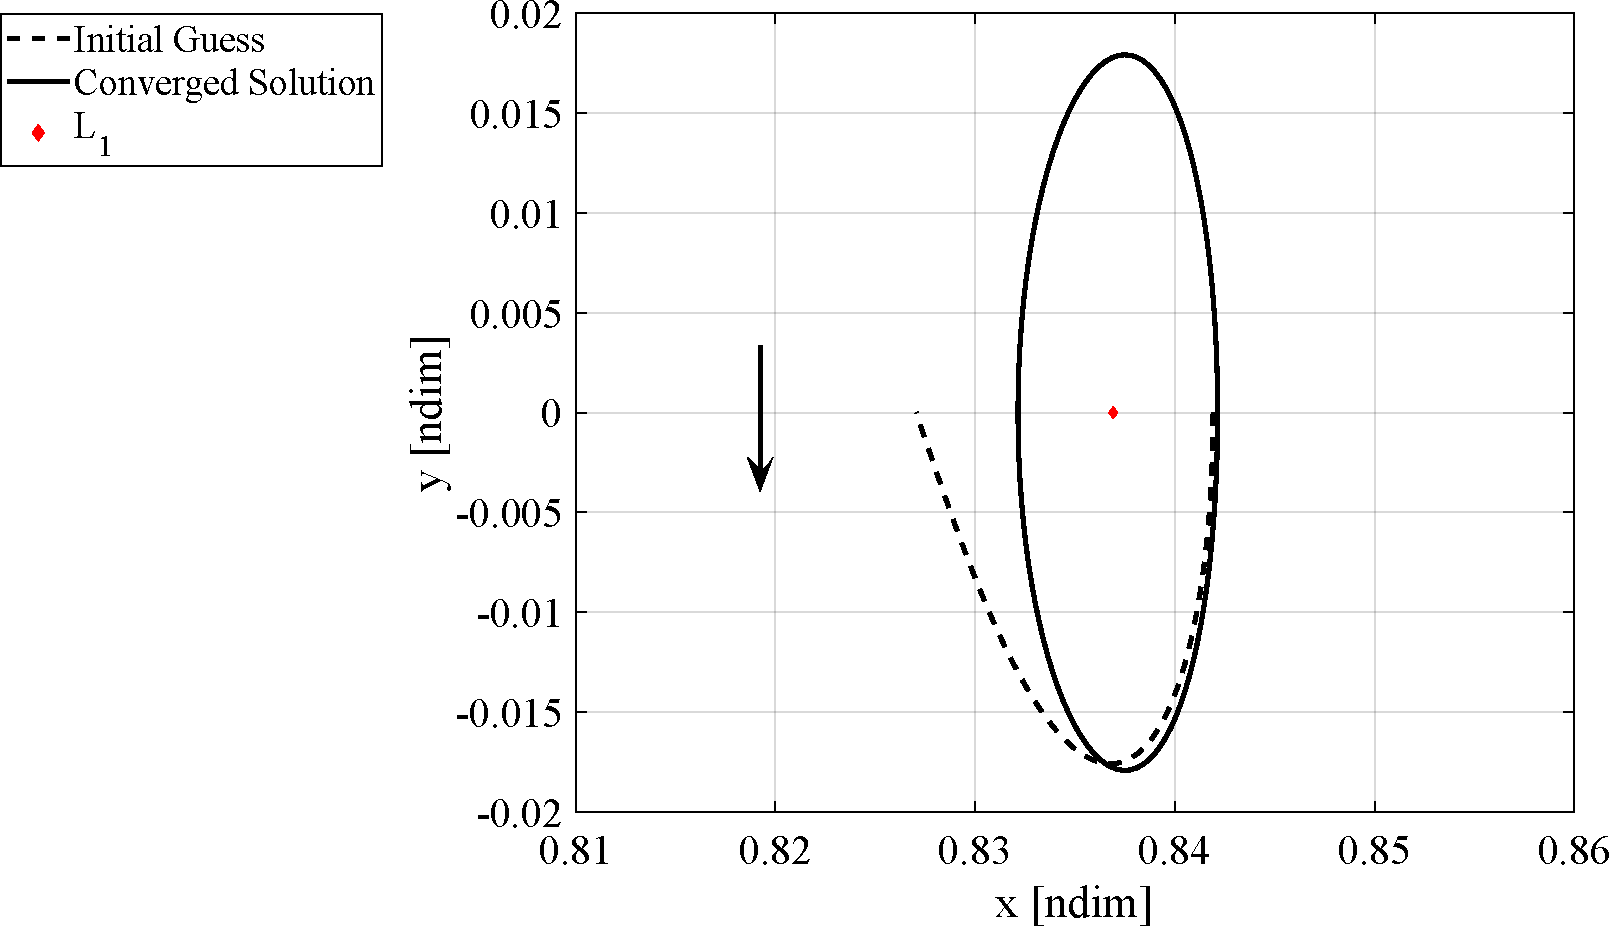
\includegraphics[width=0.75\textwidth]{figures/Lyapunov.pdf}
    \caption{Converged periodic Lyapunov orbit in the Earth-Moon barycentric rotating frame.}
    \label{fig:Lyapunov}
\end{figure}

\subsubsection{Natural Parameter Continuation}
The process described above produces a single solution near the Lagrange point. In order to compute
more solutions (orbits) in the family, especially further away from the Lagrange point where the
linear variational equations no longer apply, converged solutions can be used in a continuation
scheme to find other family members. This investigation utilizes natural parameter continuation,
where one of the parameters of a converged solution is changed by a small amount. This new guess
for an orbit is then converged, and a new solution is obtained. This continuation process can then
be repeated until the scheme reaches a natural/dynamical end or a desired orbit is reached. Natural
parameters of the orbit include (but are not limited to) components of the initial state, the
period, or the Jacobi constant. \cref{fig:L1Lyapunov} shows a large portion of the $L_{1}$ Lyapunov
family in the Earth-Moon system, continued in Jacobi constant from the orbit in
\cref{fig:Lyapunov}. Lyapunov families also exist about $L_{2}$ and $L_{3}$ and can be computed via
the same process. Since $L_{2}$ Lyapunovs are also used in this investigation, they are shown in
\cref{fig:L2Lyapunov}.

\begin{figure}[ht]
    \centering
    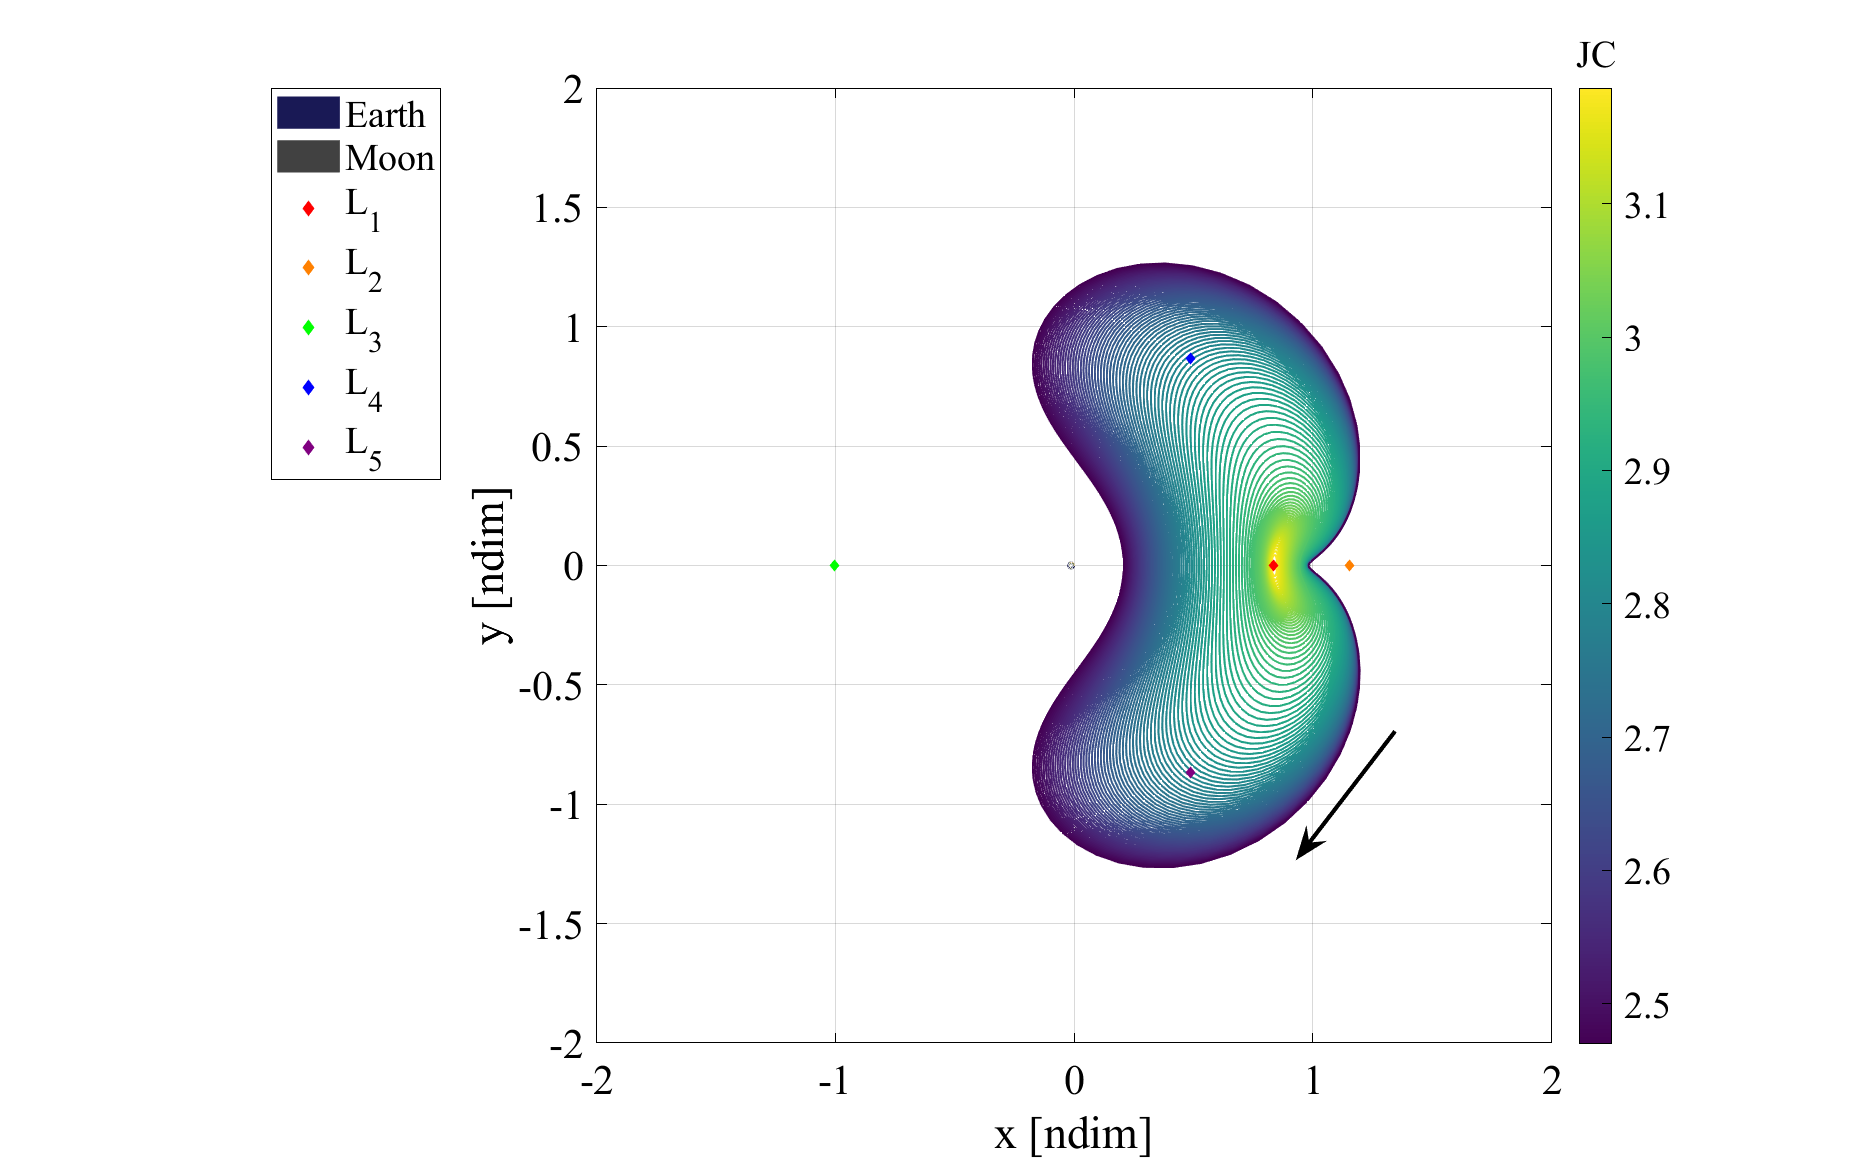
\includegraphics[width=0.9\textwidth]{figures/L1LyapunovFamily.pdf}
    \caption{Earth-Moon $L_{1}$ Lyapunov orbit family.}
    \label{fig:L1Lyapunov}
\end{figure}

\begin{figure}[ht]
    \centering
    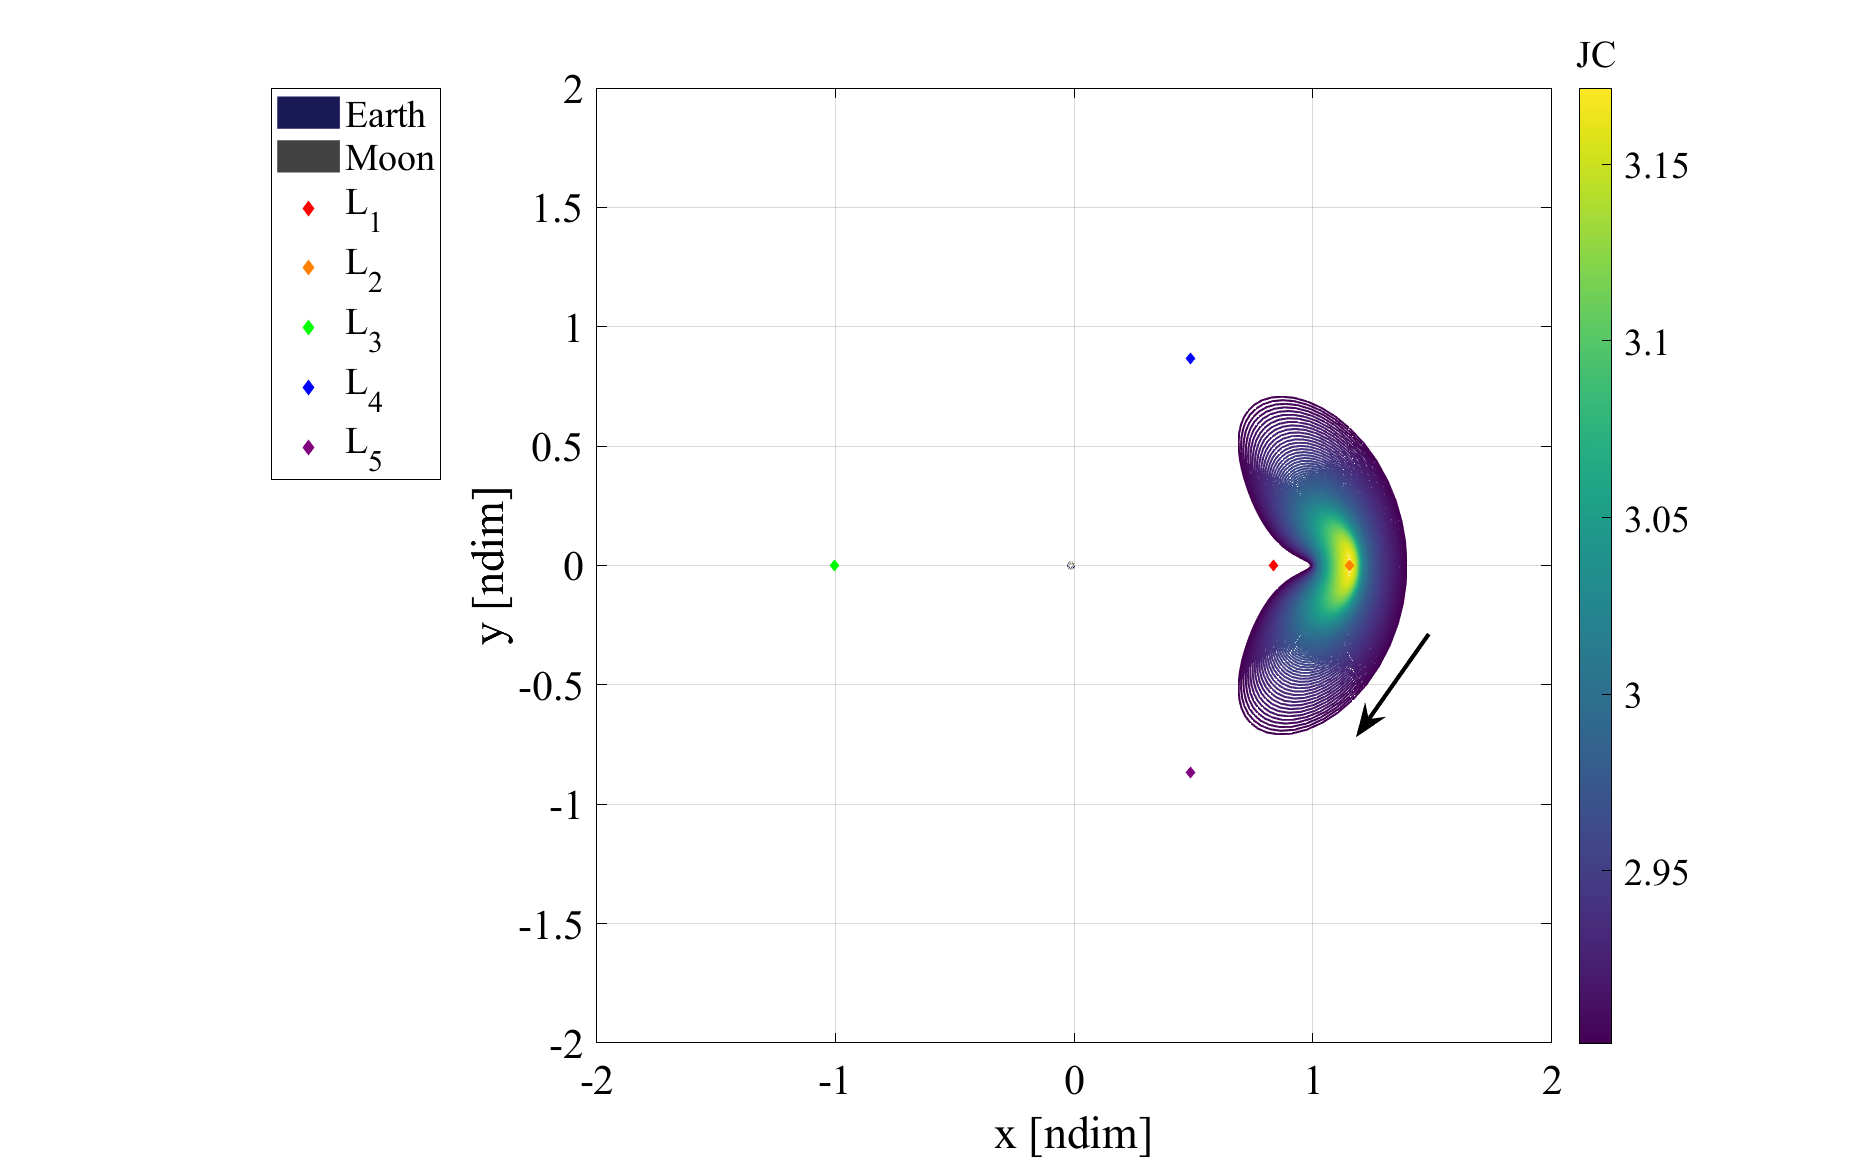
\includegraphics[width=0.9\textwidth]{figures/L2LyapunovFamily.pdf}
    \caption{Earth-Moon $L_{2}$ Lyapunov orbit family.}
    \label{fig:L2Lyapunov}
\end{figure}

\subsection{Orbital Stability}
Before discussing other orbit families, it is important to introduce orbital stability as it leads
to orbit family bifurcations and another way to generate new orbit families. Orbital stability
helps describe the characteristics of the orbit and the surrounding dynamics. The stability of an
orbit also determines the best transfer design strategies to minimize the $\Delta v$ cost. 

\phantomsection
\subsubsection{Monodromy Matrix}
The STM of one revolution of a periodic orbit in the CR3BP, $\Phi(t_{0}+\mathbb{P},t_{0})$, is
called the monodromy matrix, and discretely maps the linear growth of perturbations. Some
useful properties of the monodromy matrix are that it is symplectic, it has a determinant of $1$,
and its eigenvalues occur in reciprocal pairs\cite{ZimovanSpreen:2021}. Since the trajectory is
periodic, two of the eigenvalues (one pair) are always $1$, denoted the trivial pair, and
correspond to the trajectory's periodicity and membership in a family of solutions.

The stability of the orbit is characterized by the remaining two pairs of eigenvalues. Since the
monodromy matrix is a discrete time mapping, eigenvalues that lie within the unit circle (magnitude
less than $1$) in the complex plane are stable and those outside the unit circle are unstable.
Perturbations in the stable subspace will flow back towards the orbit, while perturbations in the
unstable subspace will depart the orbit. If the eigenvalues lie directly on the unit circle, then
the corresponding flow is in the center subspace and remains bounded around the orbit. When the
stability of an eigenvalue pair changes, it can indicate a change in the characteristics of orbits
within a family and sometimes leads to a bifurcation in the family, discussed later.

The overall stability of the orbit is then determined by all of the eigenvalues of its monodromy
matrix. If any of the eigenvaules are unstable (greater than $1$), then the orbit is considered
linearly unstable. Note that the existence of an unstable eigenvalue implies the existence of a
stable eigenvalue because of the reciprocal pairs. Otherwise, the orbit is considered marginally
stable and all of the eigenvalues reside on the unit circle. Throughout an orbit family, while the
stability of the members may change, the eigenvalues experience a smooth (but not necessarily
monotonic) evolution.

\subsubsection{Stability Index}
A variety of metrics exist to more succinctly portray the stability of orbits, rather than viewing
all of the eigenvalues. One such metric is a stability index, of which there are a variety of
definitions whose usefulness vary depending on application. In this investigation, the focus is on
just the overall stability of the orbit --- whether it is unstable or marginally stable --- so a
metric that can quickly differentiate between these behaviors suffices. Therefore, the following
definition is used\cite{Power:2019}:
\begin{equation}
    \varsigma=||\bar{\lambda}||_{\inf},
    \label{eq:stabilityindex}
\end{equation}
where $\bar{\lambda}$ is a vector of the eigenvalues of the monodromy matrix and the infinity norm
returns the magnitude of the largest (magnitude) element of the vector. With this definition,
$\varsigma>1$ indicates an unstable orbit and $\varsigma=1$ indicates one that is marginally
stable. Other definitions can be found in Zimovan Spreen's work\cite{ZimovanSpreen:2021}.

Like the eigenvalues themselves, the evolution of the stability index over an orbit family is
smooth. \cref{fig:stability} shows the stability indices for the members of the $L_{1}$ (a) and
$L_{2}$ (b) Lyapunov families from \cref{fig:L1Lyapunov} and \cref{fig:L2Lyapunov}. A larger
stability index means that the orbit hasa higher instability and perturbations will experience
faster growth. Note that all of the members of both of these families are unstable. However, there
are stability changes among individual eigenvalues within each family that can lead to
bifurcations.

\begin{figure}[ht]
    \begin{subfigure}[h]{0.4\linewidth}
        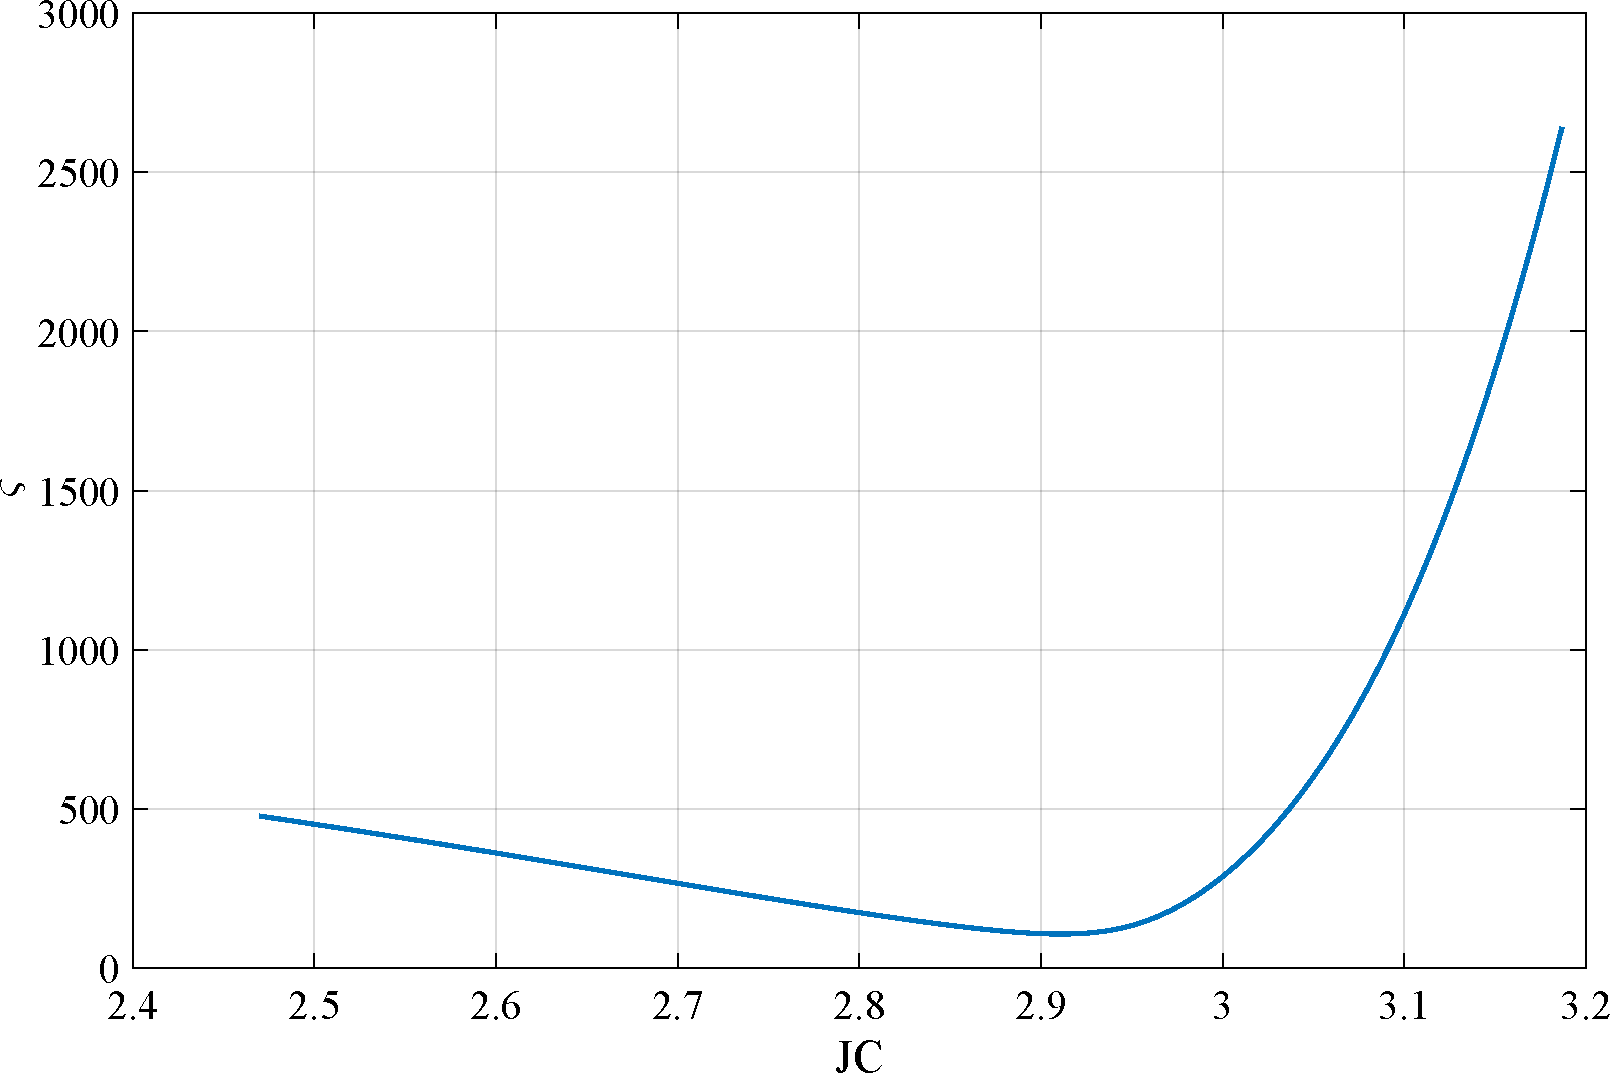
\includegraphics[width=\textwidth]{figures/L1LyapunovStability.pdf}
        \caption{$L_{1}$}
    \end{subfigure}
    \hfill
    \begin{subfigure}[h]{0.4\linewidth}
        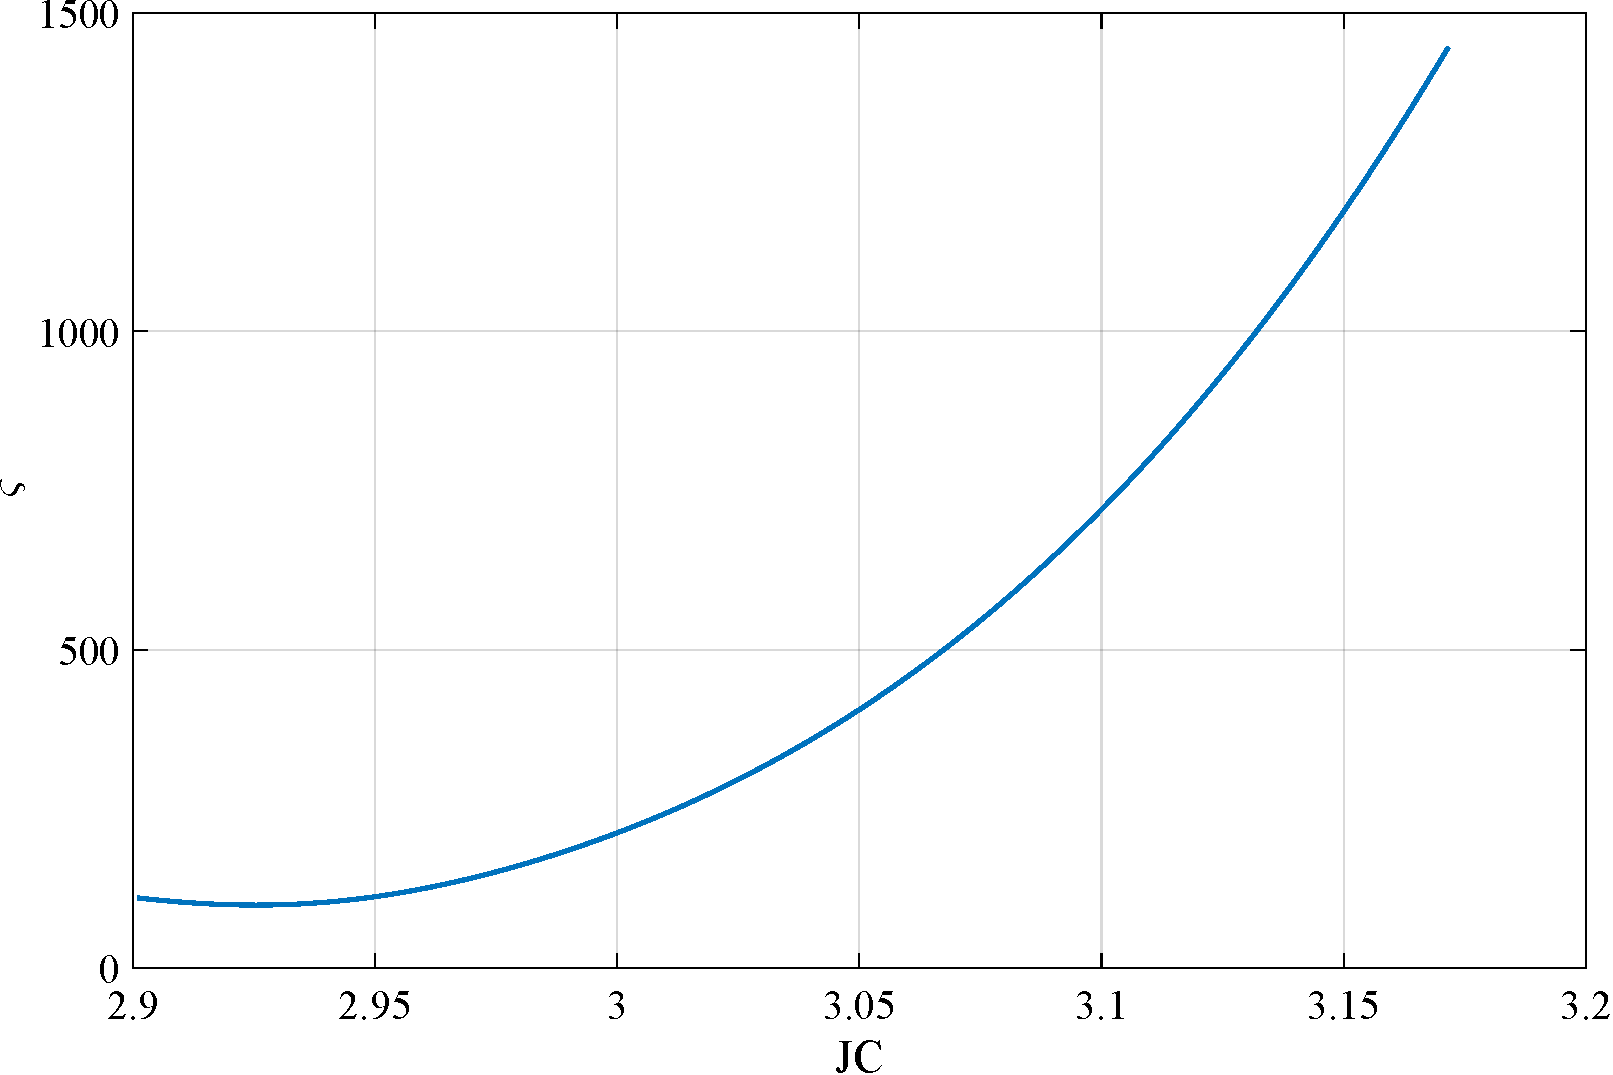
\includegraphics[width=\textwidth]{figures/L2LyapunovStability.pdf}
        \caption{$L_{2}$}
    \end{subfigure}
    \caption{Earth-Moon Lyapunov family stability index evolution.}
    \label{fig:stability}
\end{figure}

\subsubsection{Time Constant}
Another useful metric of stability is the time constant, which approximates how long it takes, in
time units or in orbit revolutions, for a perturbation to grow by a factor of $e$:
\begin{equation}
    \Upsilon=\frac{1}{\ln\varsigma},
    \label{eq:timeconstant}
\end{equation}
where the dimensions are orbit revolutions. This equation can be multiplied by the period of the
orbit $\mathbb{P}$ to produce the time constant in time units. \cref{fig:timeConstant} shows the
time constant evolution of both Lyapunov families in orbit revolutions. Note that a larger time
constant indicates that it takes longer for a perturbation, meaning that the orbit is less
unstable, and a marginally stable orbit has an infinite time constant.

\begin{figure}[ht]
    \begin{subfigure}[h]{0.4\linewidth}
        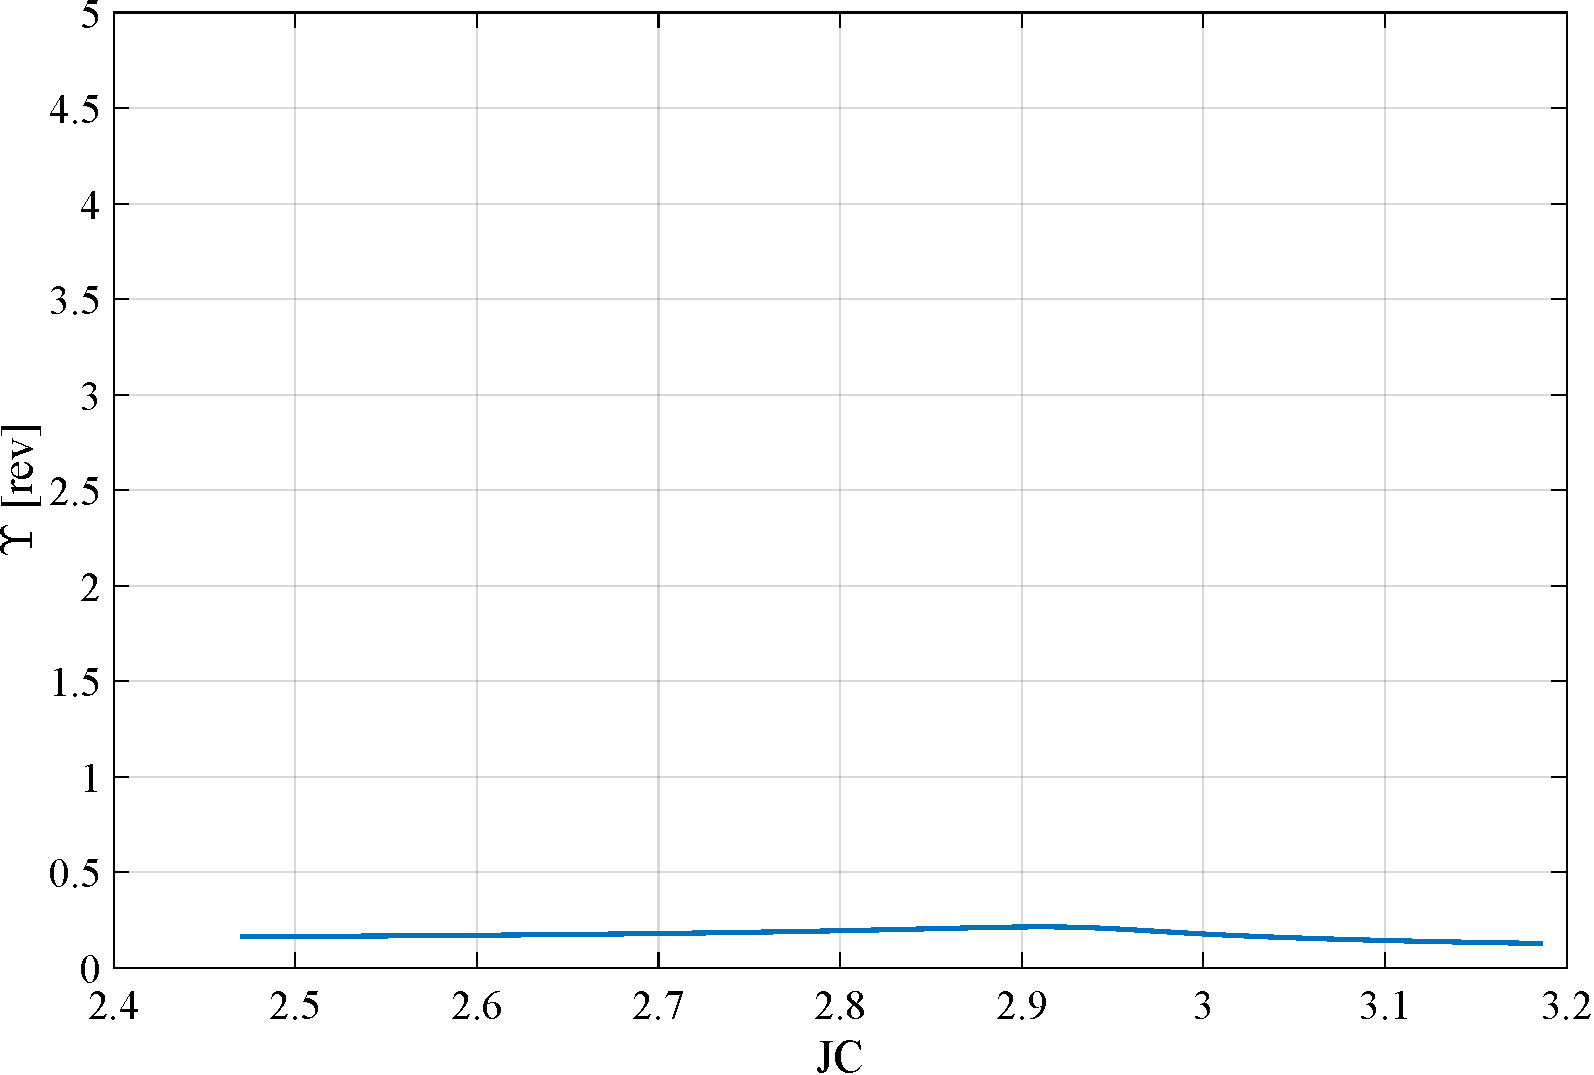
\includegraphics[width=\textwidth]{figures/L1LyapunovTimeConstant.pdf}
        \caption{$L_{1}$}
    \end{subfigure}
    \hfill
    \begin{subfigure}[h]{0.4\linewidth}
        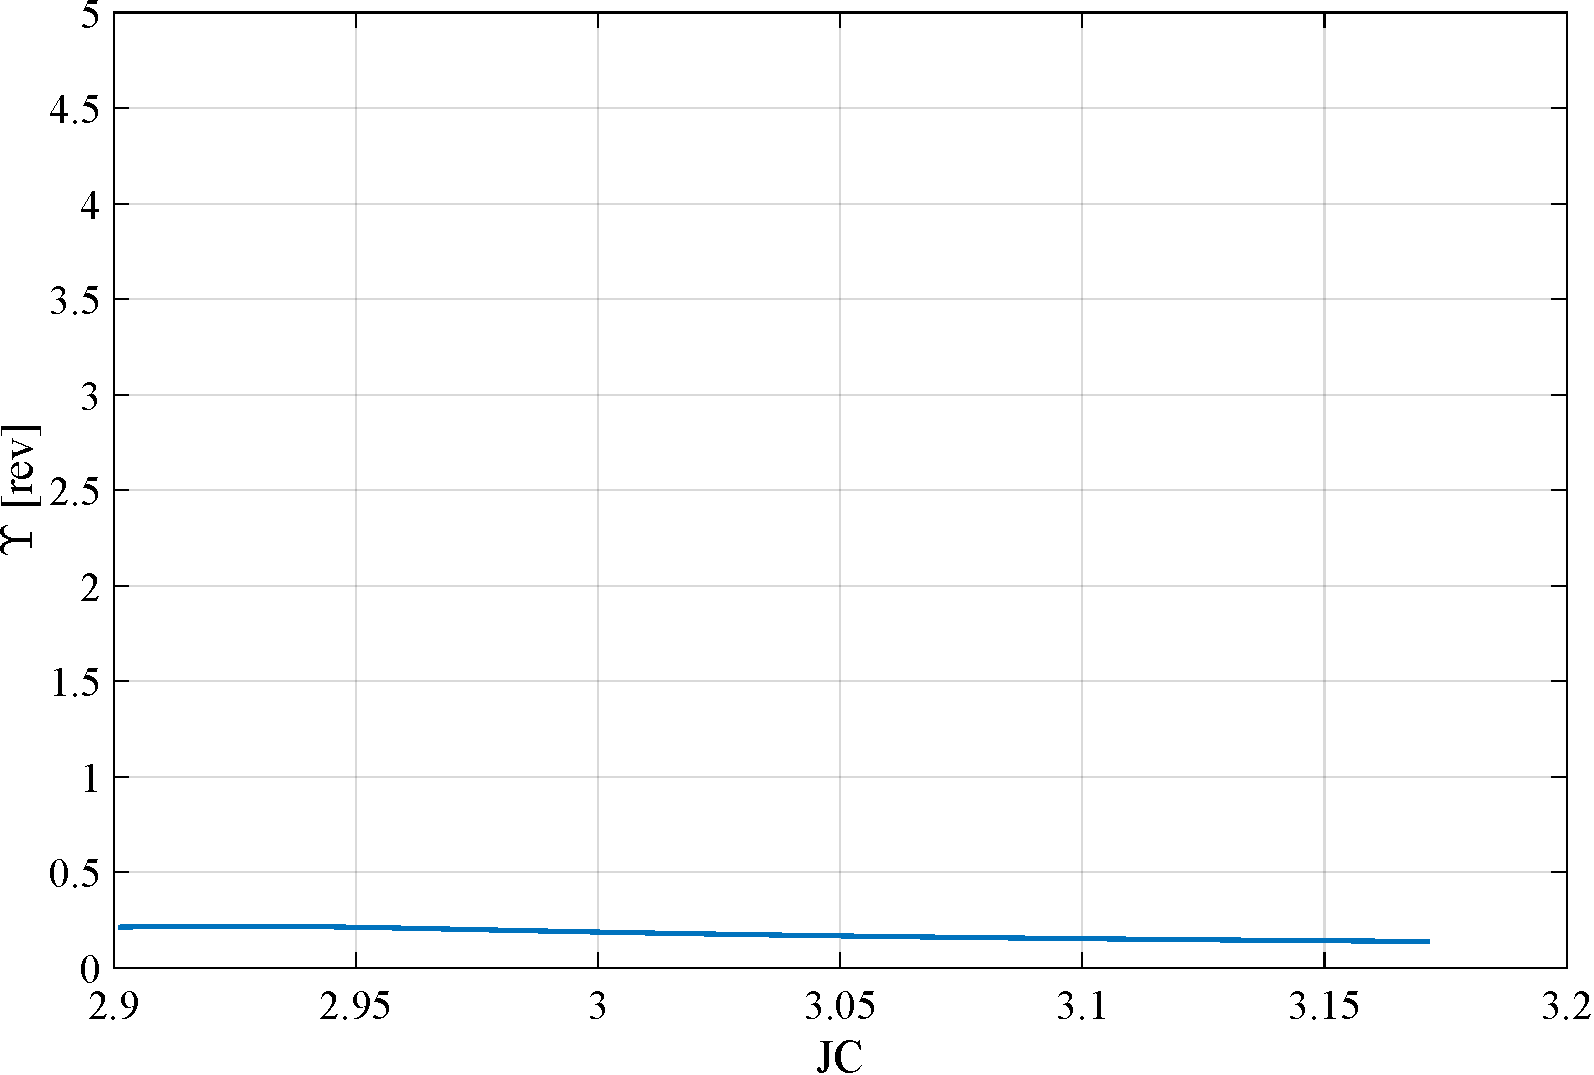
\includegraphics[width=\textwidth]{figures/L2LyapunovTimeConstant.pdf}
        \caption{$L_{2}$}
    \end{subfigure}
    \caption{Earth-Moon Lyapunov family time constant evolution.}
    \label{fig:timeConstant}
\end{figure}

\subsubsection{Bifucations}
Within the context of the CR3BP, bifurcation theory can be used to detect for changes in orbit
stability characteristics within a family that can sometimes lead to the generation of orbit
families that branch off from the original family. Zimovan Spreen provides a more thorough
analysis of how bifurcation theory can be applied to the CR3BP so only the information most
relevant to this investigation will be provided here\cite{ZimovanSpreen:2021}.

There are two main bifurcation types that are relevant to the orbits used in this analysis:
\begin{itemize}
    \item \textbf{Tangent bifurcations} occcur when an eigenvalue pair goes to $1$, either from the
    unit circle or the real axis. With a cyclic fold tangent bifurcation, which occurs at an
    extremum in Jacobi constant, the stability of the eigenvalues changes, but there is no new
    family of solutions created. Pitchfork tangent bifurcations produce two new families that have
    the same stability as the original family. The last subtype, transcritical tangent
    bifurcations, produce a new family and a change in eigenvalue stability of the original family.
    \item \textbf{Period-multiplying bifurcations} occur when an eigenvalue pair reach a root of
    $1$ ($\sqrt{1}$, $\sqrt[3]{1}$, $\sqrt[m]{1}$, etc.). In general, this produces a new family
    with a period of $m$ times the original, but not necessarily a change in stability. The most
    commonly-seen subtype is the period-doubling bifurcation, where the pair of eigenvalues meets
    at $-1$, either from the unit circle or the real axis. This results in a change in stability of
    the eigenvalues and a new family that has double the period of the original family.
\end{itemize}
There are other methods of detecting bifurcations beyond examining the evolution of the eigenvalues
such as Broucke stability or bifurcation diagrams that are also described in Zimovan
Spreen\cite{ZimovanSpreen:2021}.

\subsubsection{New Family Generation from Bifurcation}
To find the initial conditions for an orbit in a new family from a bifurcation, first the precise
bifurcating orbit (within a tolerance) must be obtained. This can be done through a simple
bisection algorithm. The Jacobian matrix of this bifurcating orbit should have an additional
nullspace compared to the other orbits in the family since another pair of eigenvalues (besides the
trivial pair) is at $1$. Note that for a period-multiplying bifurcation, the orbit must be
propagated for $m$ revolutions to obtain the proper Jacobian matrx. When this is the case, one of
the nullspace vectors points in the direction of continuing the old family, while the other vector
indicates a direction for the new family.

Using a singular value decomposition (SVD), this new nullspace direction can be identified by the
right singular vector of $DF$ that corresponds to the additional nullspace. Stepping in this
direction from the bifurcating orbit's initial conditions and correcting for a periodic solution
should result in a new periodic orbit belonging to the new family. This approach is also known as
pseudo-arclength continuation and the new member can then be continued using any scheme to obtain
the new family.

\subsection{Halo Orbit Families}
\phantomsection
\subsubsection{A Halo Targeter}
Similar to Lyapunov orbits, halo orbits are symmetric about the $xz$-plane although they are
spatial in the rotating frame and not limited to the $xy$-plane. This again allows for
targeting only half of the periodic orbit, from one perpendicular crossing to the next. Since there
is now a $z$-component to the orbits, it is helpful to introduce a new free variable and constraint
for the halo targeter:
\begin{equation}
    \Xbar=\begin{bmatrix}   x_{0}   &   z_{0}   &   \ydot_{0}   &   \tau    \end{bmatrix}^{T},
    \label{eq:halofreevar}
\end{equation}
\begin{equation}
    \Fbar(\Xbar)=\begin{bmatrix}    y_{f}   &   \xdot_{f}   &   \zdot_{f}   &   C-C_{d} \end{bmatrix}^{T}=\zerobar,
    \label{eq:haloconst}
\end{equation}
\begin{equation}
    DF(\Xbar)=\begin{bmatrix}   \phi_{21}                                                                   &   \phi_{23}                                               &   \phi_{25}                                   &   \ydot_{f}                               \\
                                \phi_{41}                                                                   &   \phi_{43}                                               &   \phi_{45}                                   &   \xddot_{f}                              \\
                                \phi_{61}                                                                   &   \phi_{63}                                               &   \phi_{65}                                   &   \zddot_{f}                              \\
                                2x_{0}-\frac{2(x_{0}+\mu)(1-\mu)}{d^{3}}-\frac{2\mu(x_{0}-1+\mu)}{r^{3}}    &   -\frac{2z_{0}(1-\mu)}{d^{3}}-\frac{2z_{0}\mu}{r^{3}}    &   -2\ydot_{0}                                 &   0                                       \end{bmatrix}.
    \label{eq:halojacobian}
\end{equation}
The result of this targeting will provide the initial state ($y_{0}=\xdot_{0}=\zdot_{0}=0$) and
half of the propagation time for a periodic halo orbit.

\subsubsection{Converged Halo Families}
The initial guess for a halo orbit comes from a bifurcating orbit in a Lyapunov family. At
$C\approx3.174352$, the $L_{1}$ Lyapunov family has a tangent bifurcation and the $L_{1}$ halo
family is formed. The pseudo-arclength method for generating an initial guess can be used as
described above to obtain the initial guess for the initial state, propagation time, and Jacobi
constant. Using natural parameter continuation, more of the family is produced, shown in
\cref{fig:L1Halo}. Since the Lyapunov orbit can bifurcate above or below the $xy$-plane, two halves
of the family are formed. \cref{fig:L1Halo} is denoted the $L_{1}$ southern halos because most of
the orbit is spent south (in the rotating frame) of the Moon.

\begin{figure}[ht]
    \centering
    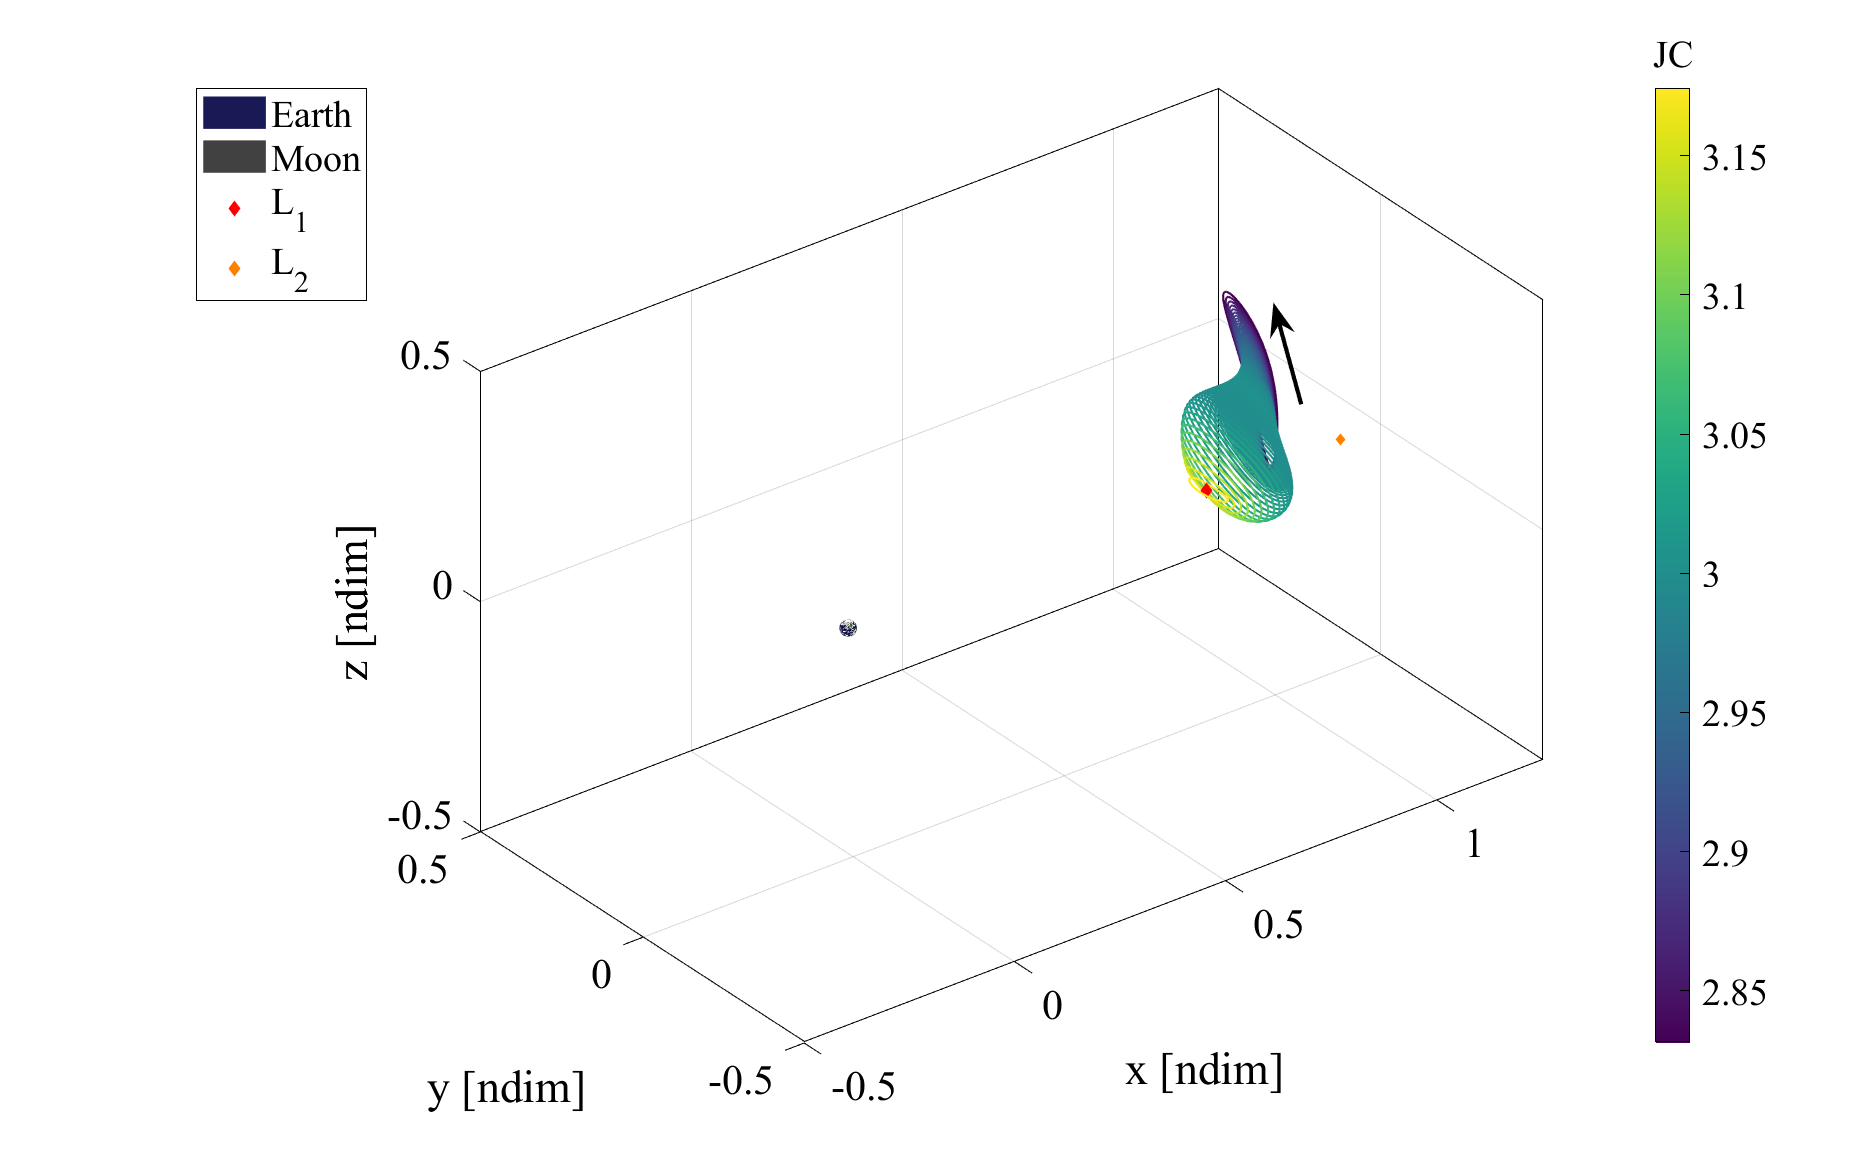
\includegraphics[width=0.9\textwidth]{figures/L1HaloFamily.pdf}
    \caption{Earth-Moon $L_{1}$ southern halo orbit family.}
    \label{fig:L1Halo}
\end{figure}

\cref{fig:L2Halo} shows the $L_{2}$ southern halo family, generated in the same way as the $L_{1}$
halos but from the $L_{2}$ Lyapunov family. Note that these halo families are not monotonic in
Jacobi constant. The stability indices for both families are shown in \cref{fig:haloStability}.
$L_{3}$ halos also exist, but are not used in this investigation.

\begin{figure}[ht]
    \centering
    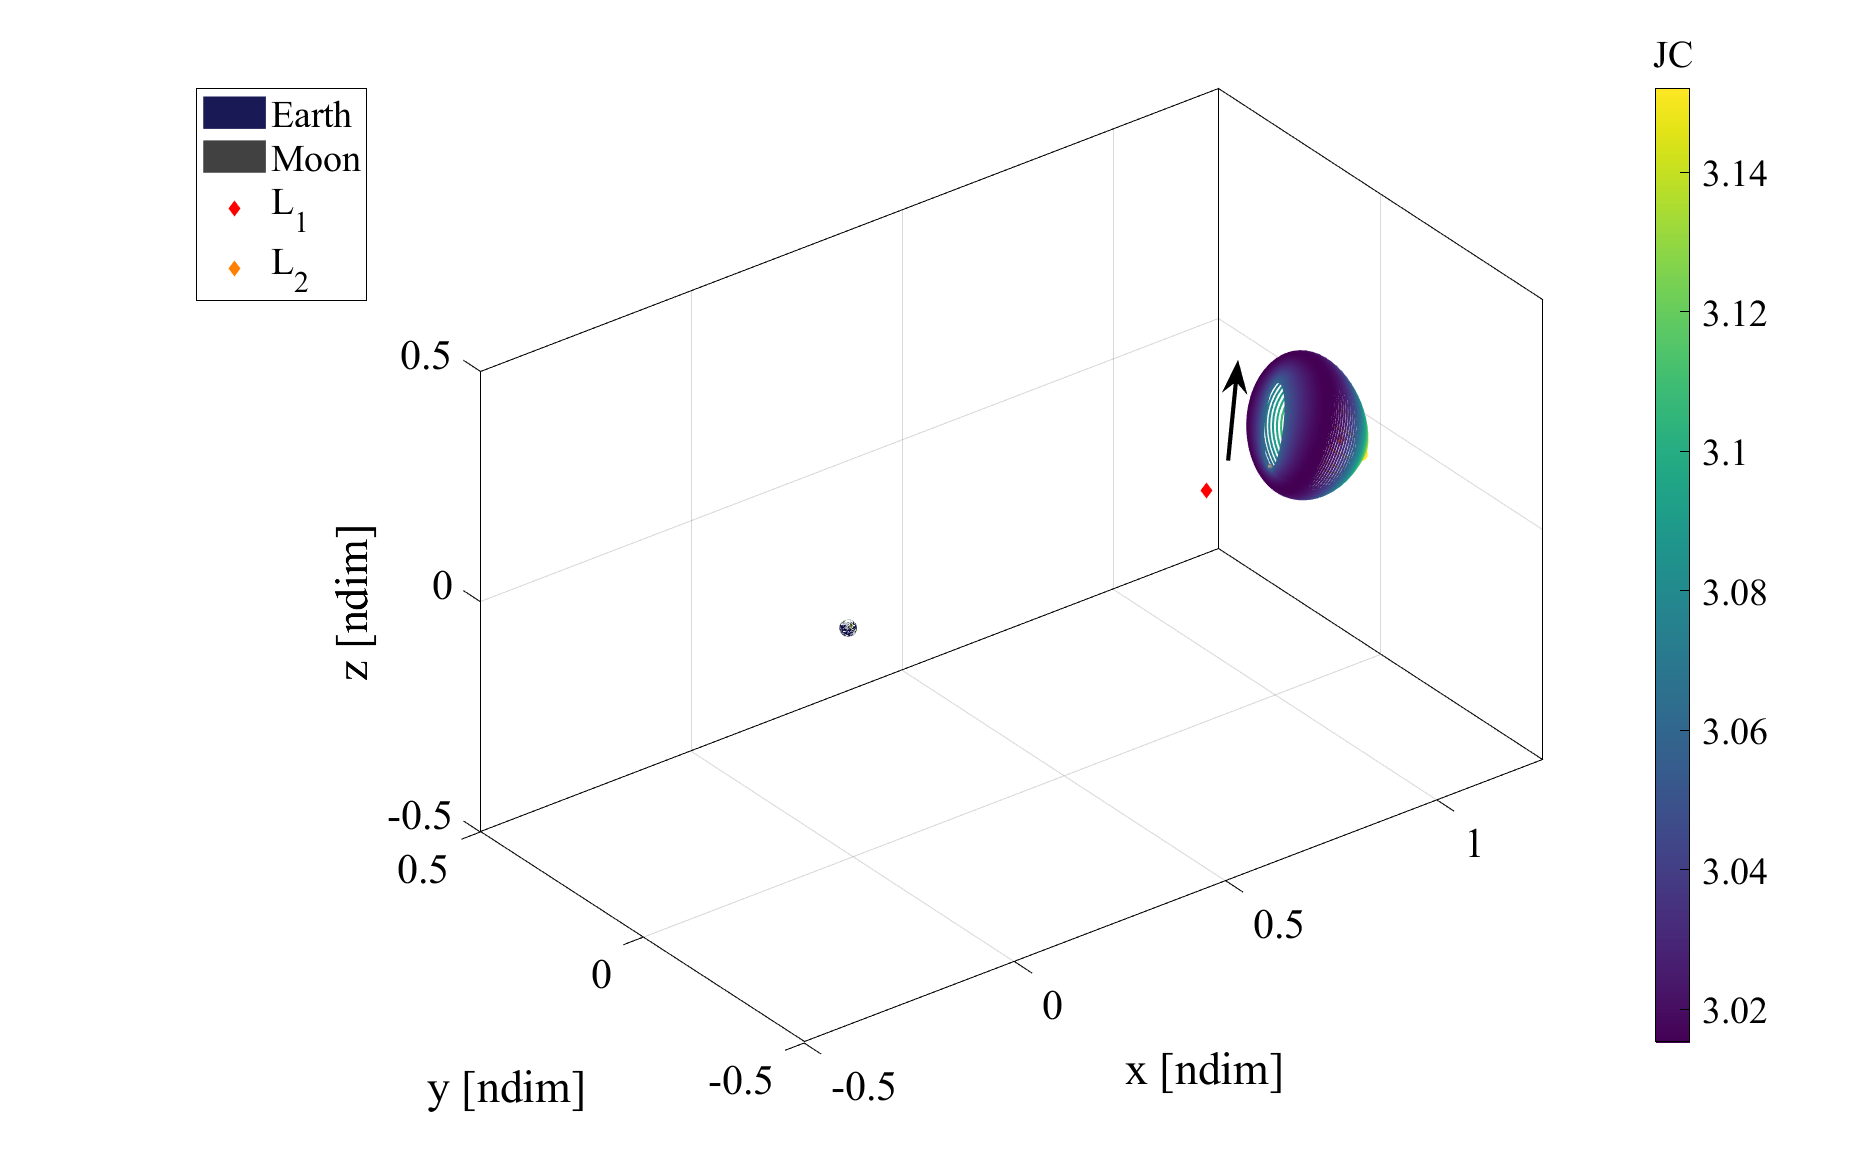
\includegraphics[width=0.9\textwidth]{figures/L2HaloFamily.pdf}
    \caption{Earth-Moon $L_{2}$ southern halo orbit family.}
    \label{fig:L2Halo}
\end{figure}

\begin{figure}[ht]
    \begin{subfigure}[h]{0.4\linewidth}
        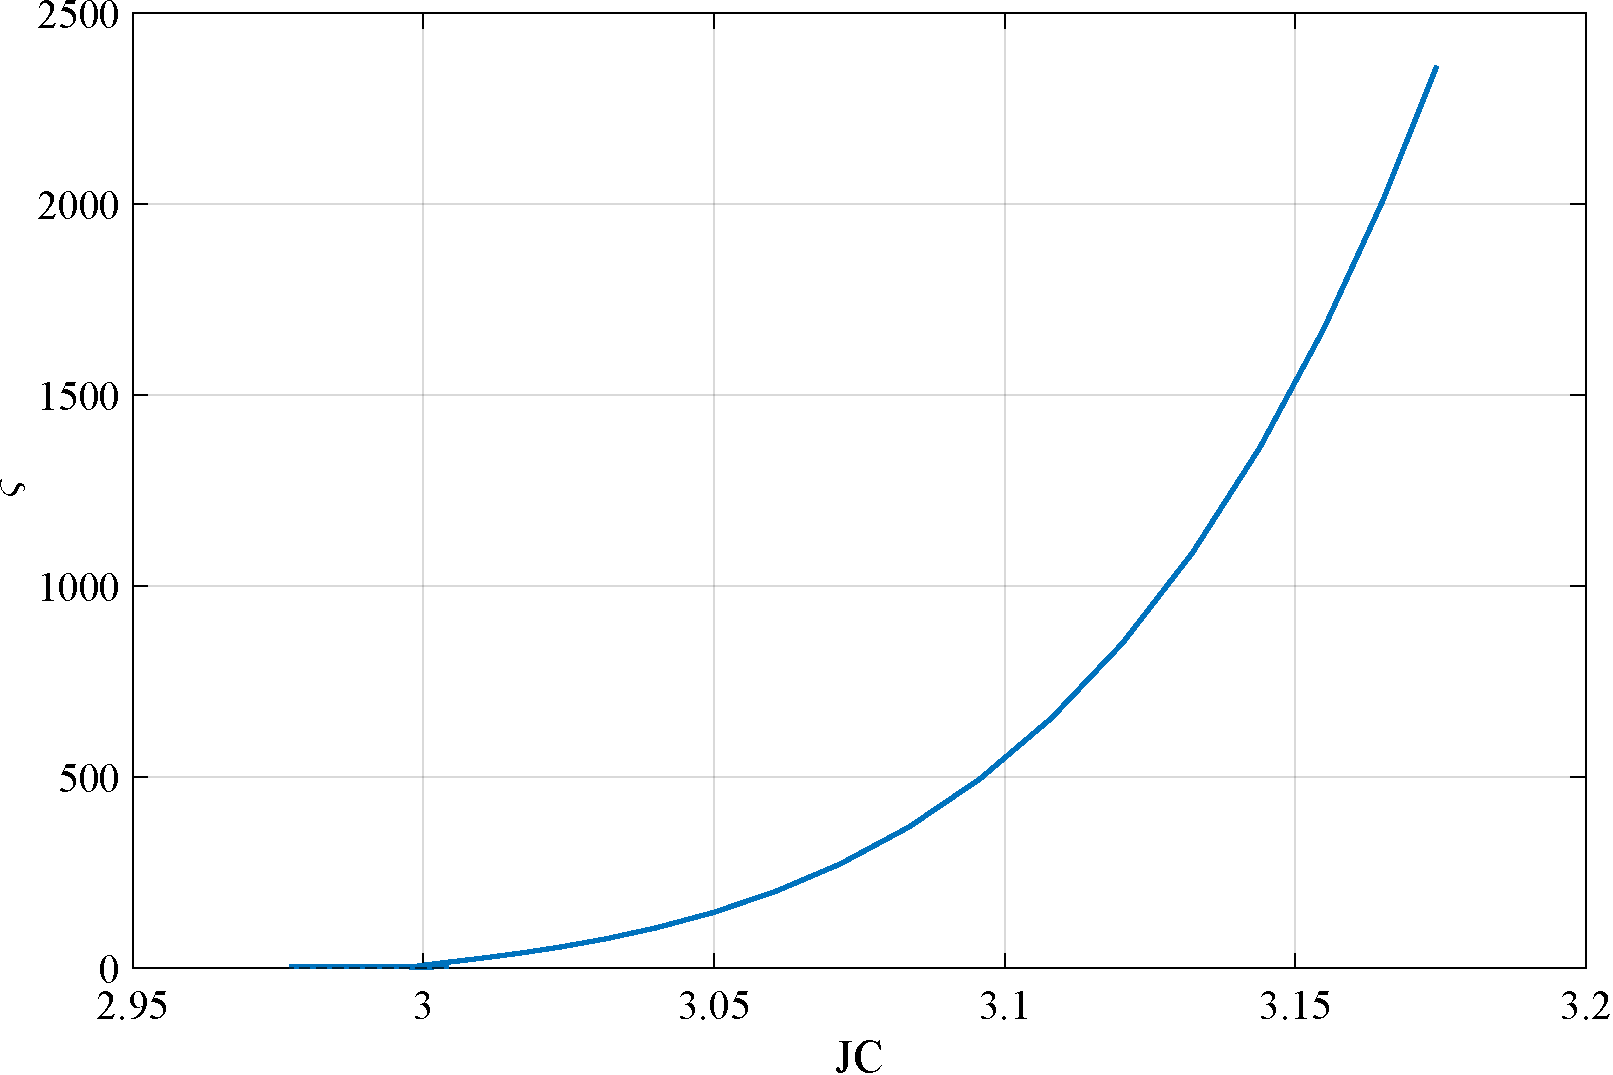
\includegraphics[width=\textwidth]{figures/L1HaloStability.pdf}
        \caption{$L_{1}$}
    \end{subfigure}
    \hfill
    \begin{subfigure}[h]{0.4\linewidth}
        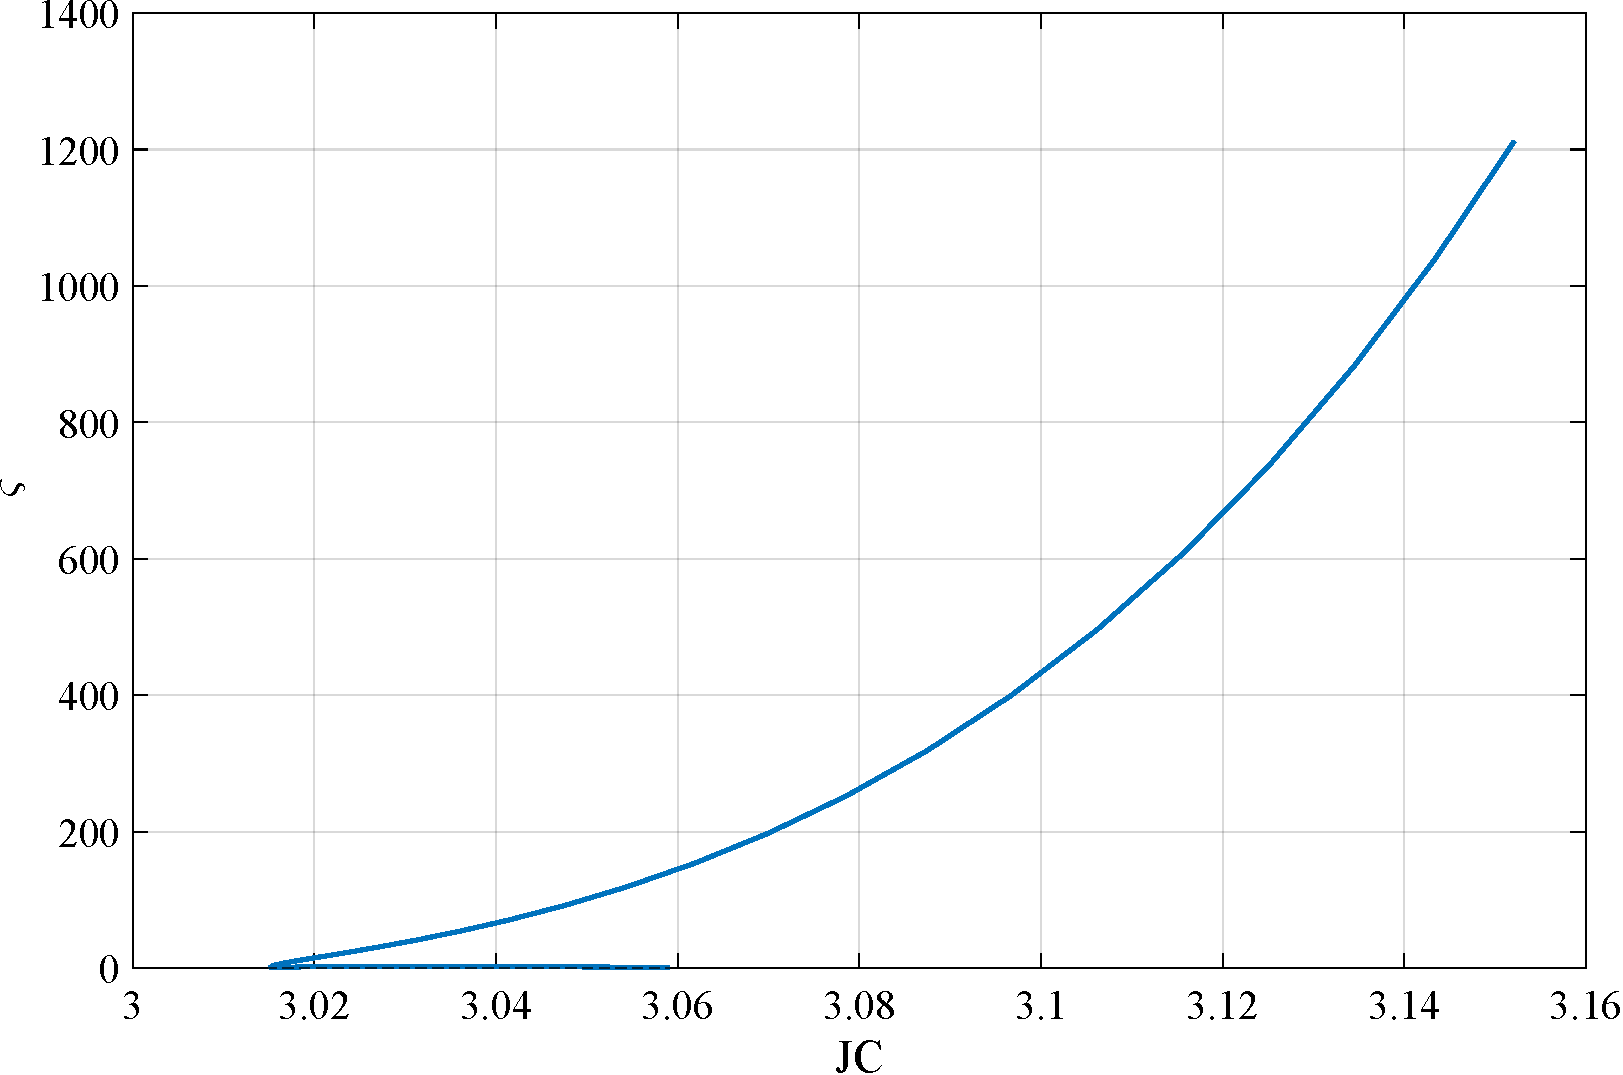
\includegraphics[width=\textwidth]{figures/L2HaloStability.pdf}
        \caption{$L_{2}$}
    \end{subfigure}
    \caption{Earth-Moon Halo family stability index evolution.}
    \label{fig:haloStability}
\end{figure}

\subsection{Axial Orbit Families}
\phantomsection
\subsubsection{An Axial Targeter}
Another spatial orbit family, the axial orbits, comes from a different tangent bifurcation in the
Lyapunov families. These orbits have symmetry only about the $x$-axis; therefore, the perpendicular
crossings must lie on the $x$-axis, unlike the halo orbits:
\begin{equation}
    \Xbar=\begin{bmatrix}   x_{0}   &   \ydot_{0}   &   \zdot_{0}   &   \tau    \end{bmatrix}^{T},
    \label{eq:axialfreevar}
\end{equation}
\begin{equation}
    \Fbar(\Xbar)=\begin{bmatrix}    y_{f}   &   z_{f}   &   \xdot_{f}   &   C-C_{d} \end{bmatrix}^{T}=\zerobar,
    \label{eq:axialconst}
\end{equation}
\begin{equation}
    DF(\Xbar)=\begin{bmatrix}   \phi_{21}                                                                   &   \phi_{25}   &   \phi_{26}   &   \ydot_{f}   \\
                                \phi_{31}                                                                   &   \phi_{35}   &   \phi_{36}   &   \zdot_{f}   \\
                                \phi_{41}                                                                   &   \phi_{45}   &   \phi_{46}   &   \xddot_{f}  \\
                                2x_{0}-\frac{2(x_{0}+\mu)(1-\mu)}{d^{3}}-\frac{2\mu(x_{0}-1+\mu)}{r^{3}}    &   -2\ydot_{0} &   -2\zdot_{0} &   0           \end{bmatrix}.
    \label{eq:axialjacobian}
\end{equation}
The result of this targeting will provide the initial state ($y_{0}=z_{0}=\xdot_{0}=0$) and half of
the propagation time for a periodic axial orbit.

\subsubsection{Converged Axial Families}
From the methods used to obtain the halo families, the $L_{1}$ and $L_{2}$ axial families can also
be obtained, shown in \cref{fig:L1Axial} and \cref{fig:L2Axial} respectively. Similar to the halo
orbits, there are two halves to the family that can be obtained by bifurcating above or below the
$xy$-plane, making these the $L_{1}$ northeast and $L_{2}$ northwest axial families. Their
stability indices follow in \cref{fig:axialStability}. Again, there is an $L_{3}$ axial family, but
it is not used in this investigation.

\begin{figure}[ht]
    \centering
    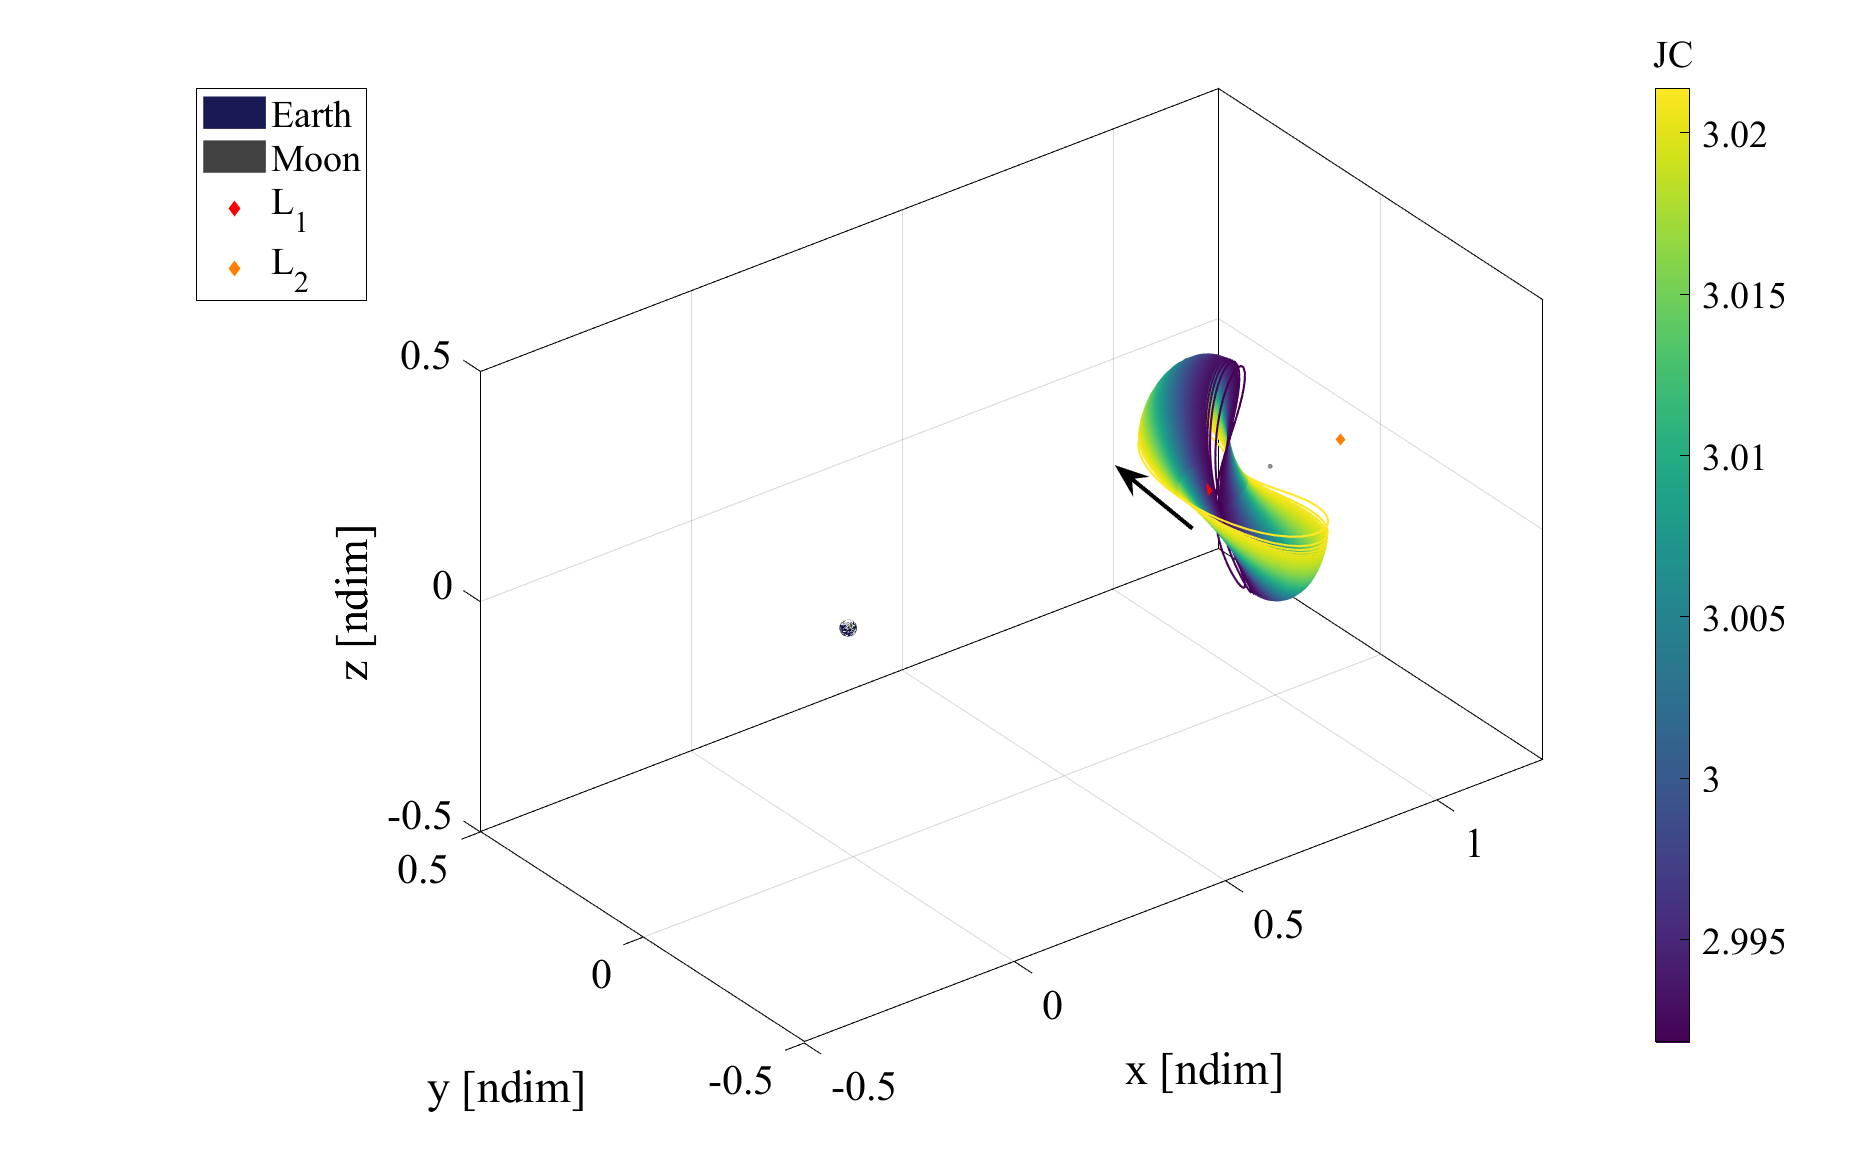
\includegraphics[width=0.9\textwidth]{figures/L1AxialFamily.pdf}
    \caption{Earth-Moon $L_{1}$ northeast axial orbit family.}
    \label{fig:L1Axial}
\end{figure}

\begin{figure}[ht]
    \centering
    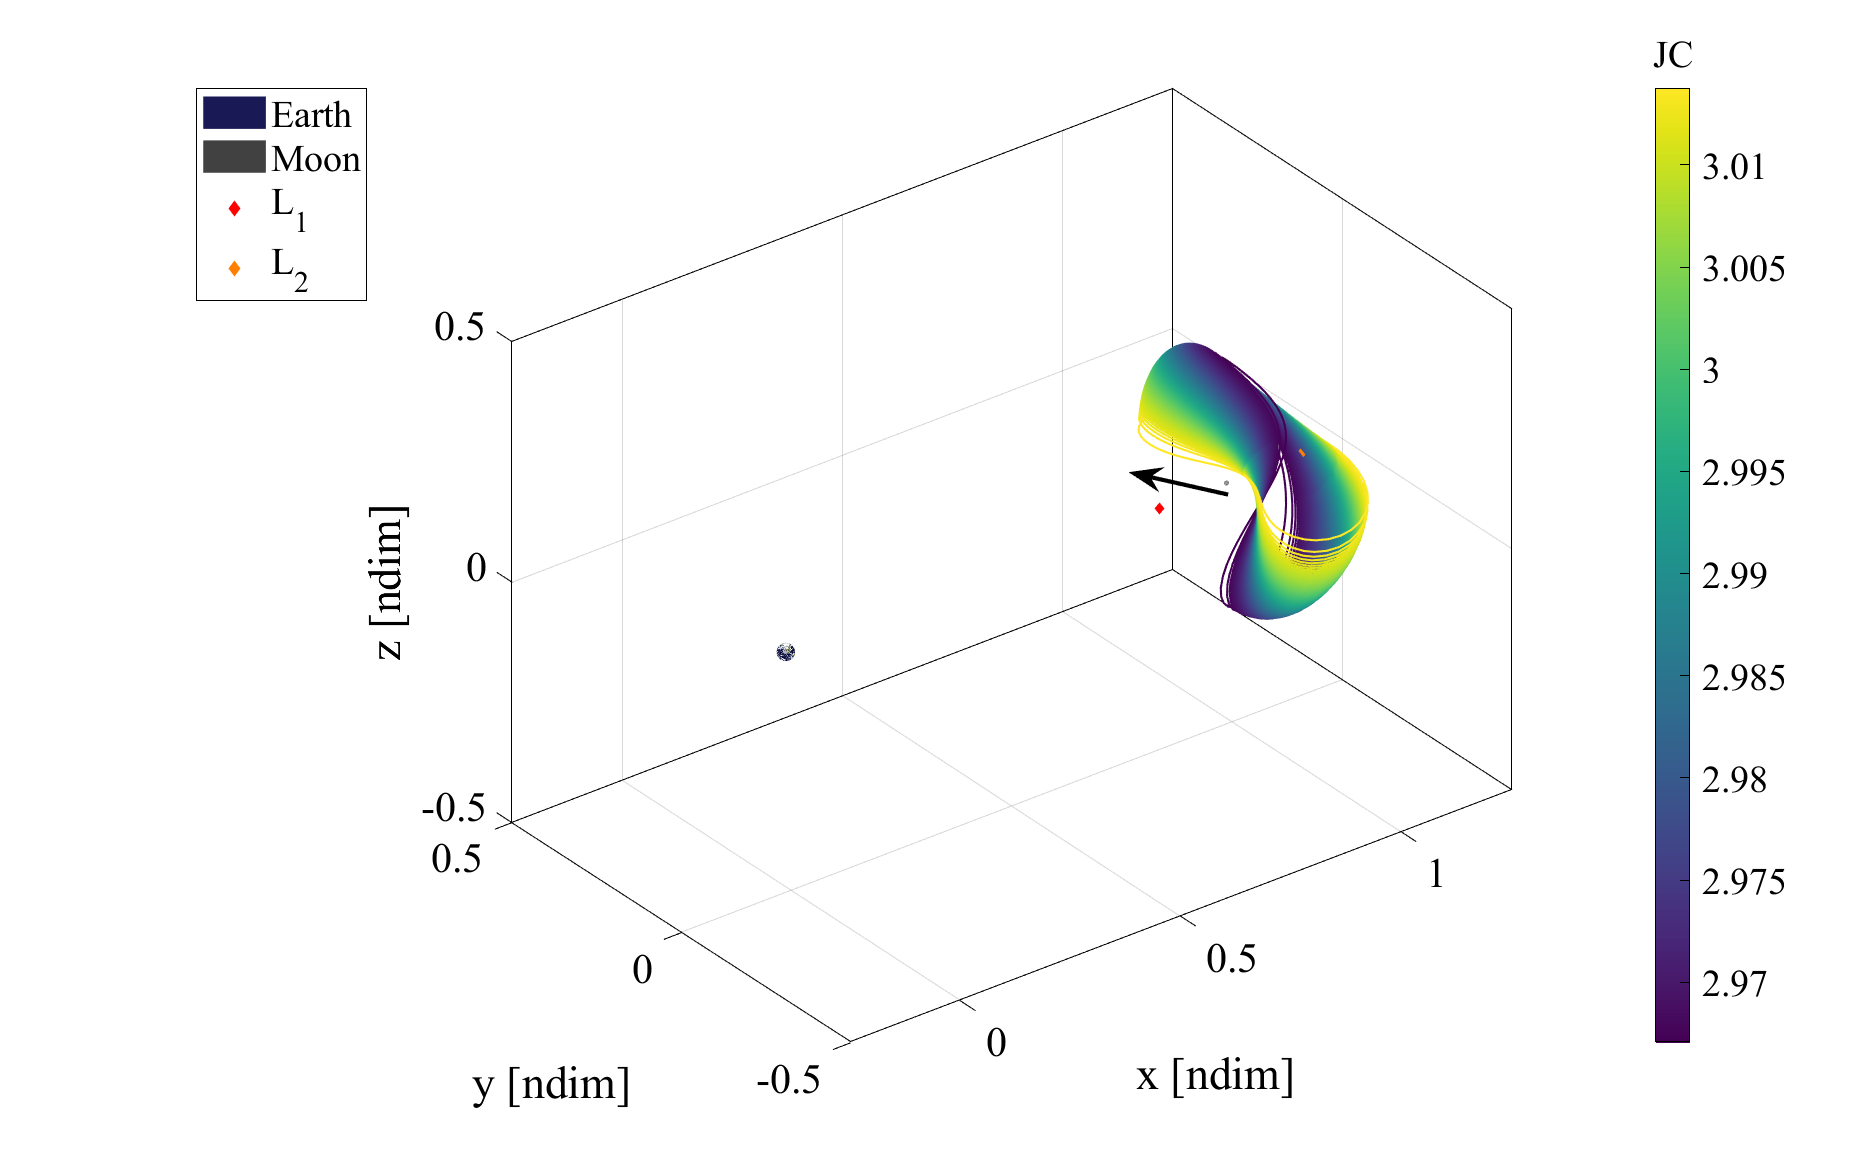
\includegraphics[width=0.9\textwidth]{figures/L2AxialFamily.pdf}
    \caption{Earth-Moon $L_{2}$ northwest axial orbit family.}
    \label{fig:L2Axial}
\end{figure}

\begin{figure}[ht]
    \begin{subfigure}[h]{0.4\linewidth}
        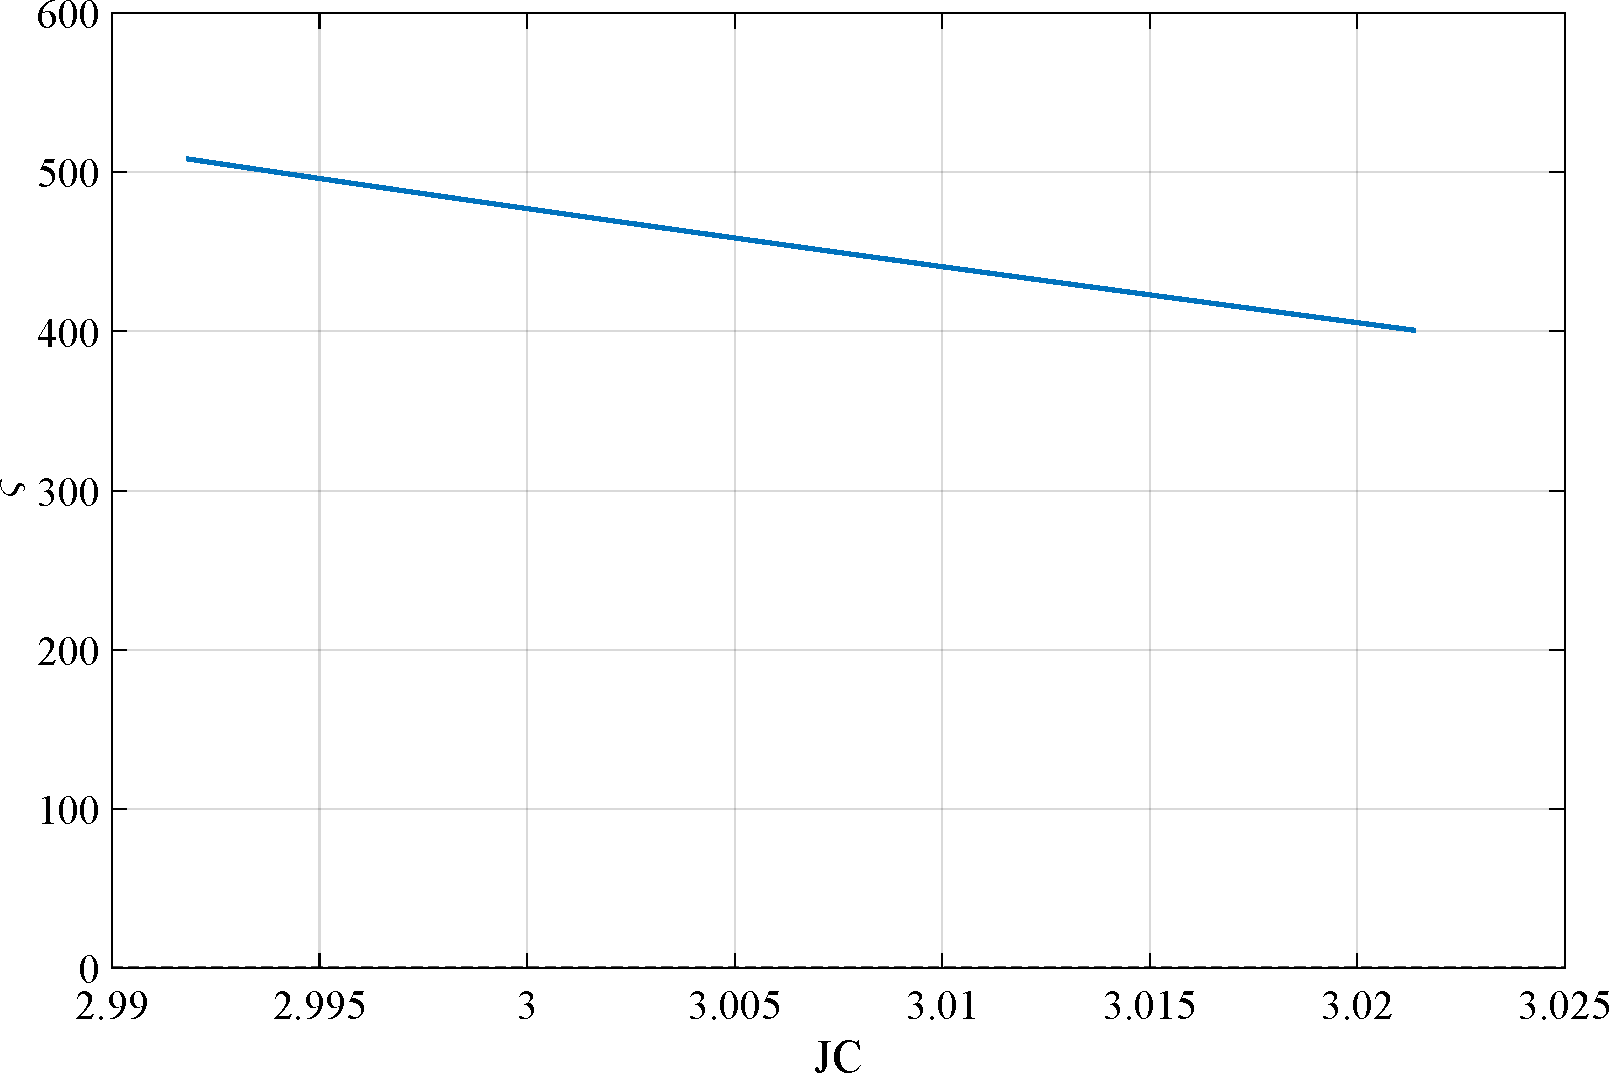
\includegraphics[width=\textwidth]{figures/L1AxialStability.pdf}
        \caption{$L_{1}$}
    \end{subfigure}
    \hfill
    \begin{subfigure}[h]{0.4\linewidth}
        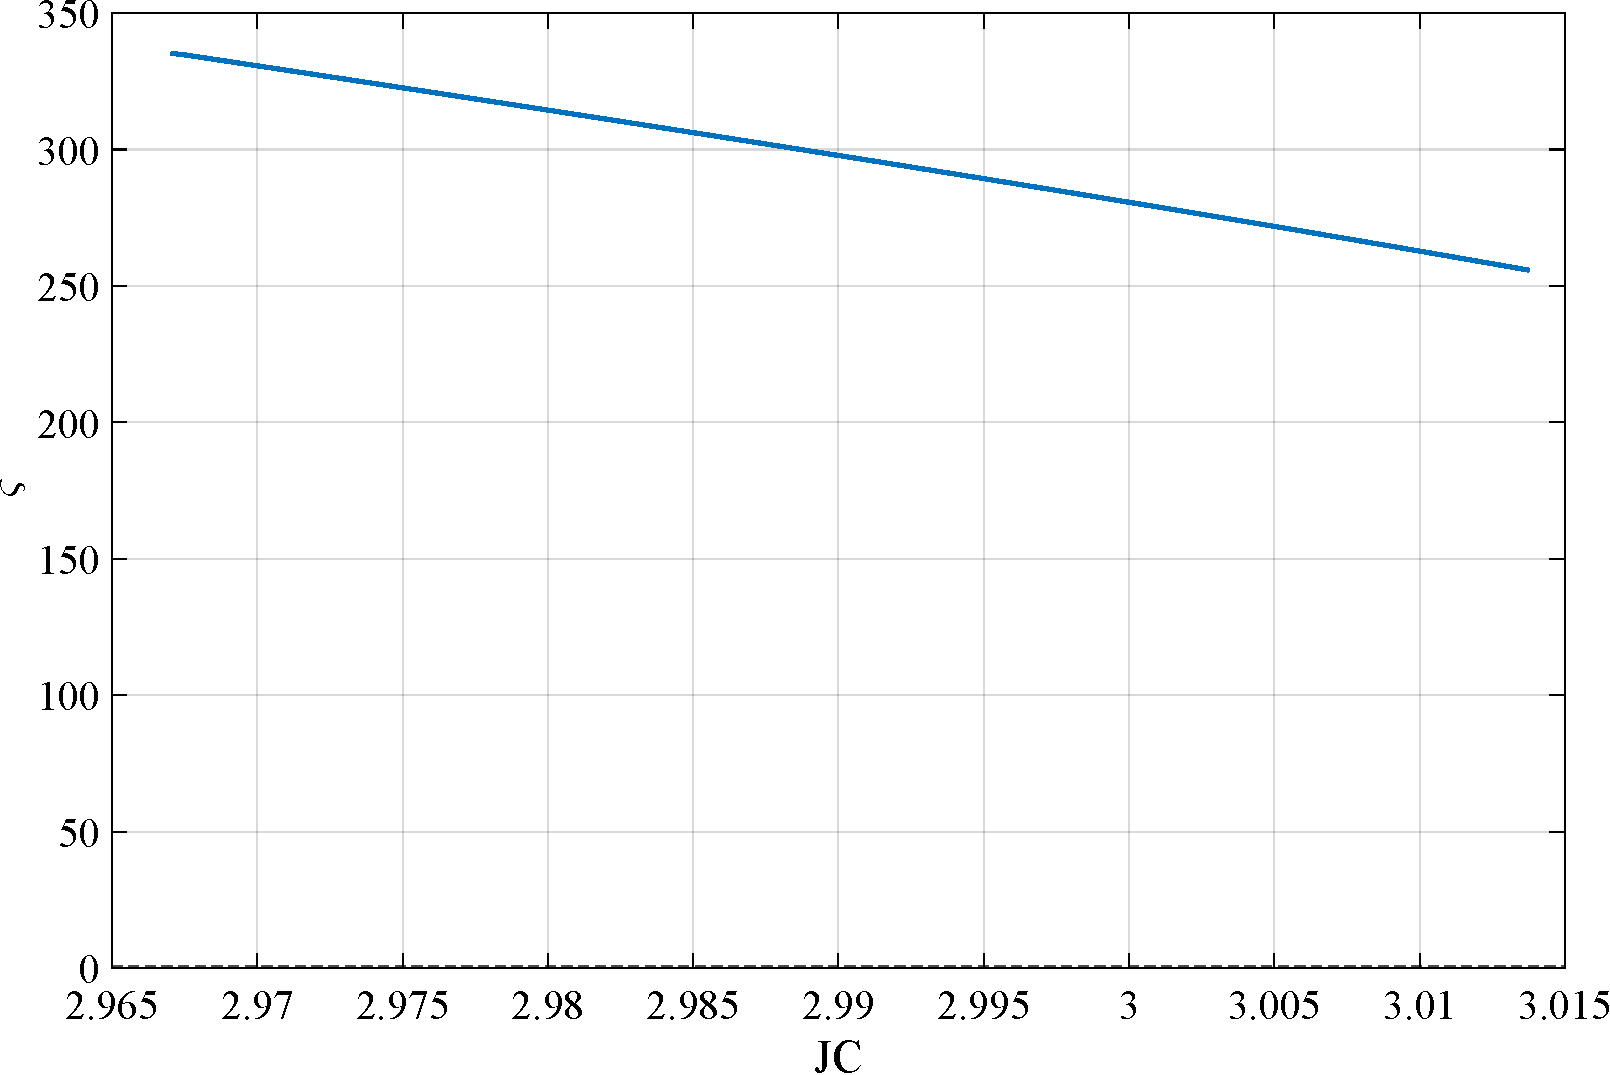
\includegraphics[width=\textwidth]{figures/L2AxialStability.pdf}
        \caption{$L_{2}$}
    \end{subfigure}
    \caption{Earth-Moon axial family stability index evolution.}
    \label{fig:axialStability}
\end{figure}

\subsection{Vertical Orbit Families}
\phantomsection
\subsubsection{A Vertical Targeter}
Vertical orbits benefit from double symmetry about both the $xz$- and $xy$-planes. This allows for
targeting of only a quarter of the orbit, with a perpendicular crossing of the $xz$-plane on one
end of the arc and a perpendicular crossing of the $x$-axis on the other. Starting from the
$xz$-plane crossing:
\begin{equation}
    \Xbar=\begin{bmatrix}   x_{0}   &   z_{0}   &   \ydot_{0}   &   \tau    \end{bmatrix}^{T},
    \label{eq:verticalfreevar}
\end{equation}
\begin{equation}
    \Fbar(\Xbar)=\begin{bmatrix}    y_{f}   &   z_{f}   &   \xdot_{f}   &   C-C_{d} \end{bmatrix}^{T}=\zerobar,
    \label{eq:verticalconst}
\end{equation}
\begin{equation}
    DF(\Xbar)=\begin{bmatrix}   \phi_{21}                                                                   &   \phi_{23}                                               &   \phi_{25}   &   \ydot_{f}   \\
                                \phi_{31}                                                                   &   \phi_{33}                                               &   \phi_{35}   &   \zdot_{f}   \\
                                \phi_{41}                                                                   &   \phi_{43}                                               &   \phi_{45}   &   \xddot_{f}  \\
                                2x_{0}-\frac{2(x_{0}+\mu)(1-\mu)}{d^{3}}-\frac{2\mu(x_{0}-1+\mu)}{r^{3}}    &   -\frac{2z_{0}(1-\mu)}{d^{3}}-\frac{2z_{0}\mu}{r^{3}}    &   -2\ydot_{0} &   0           \end{bmatrix}.
    \label{eq:verticaljacobian}
\end{equation}
The result of this targeting will provide the initial state ($y_{0}=\xdot_{0}=\zdot_{0}=0$) at the
perpendicular crossing of the $xz$-plane (top/bottom of the orbit) and one quarter of the
propagation time for a periodic vertical orbit.

\subsubsection{Converged Vertical Families}
The vertical orbit family bifurcates from the end of the axial family, when the axial orbit
intersects itself and resembles a figure-eight. Stepping in one direction shrinks the orbits as the
family collapses down to its origin Lagrange point. The other direction expands the orbits until
they look like clam shells, demonstrated for the $L_{1}$ family in \cref{fig:L1Vertical}. Similar
behavior occurs with the $L_{2}$ vertical family in \cref{fig:L2Vertical}.
\cref{fig:verticalStability} shows the stability indices for these two families; $L_{3}$ verticals
are not used in this investigation.

\begin{figure}[ht]
    \centering
    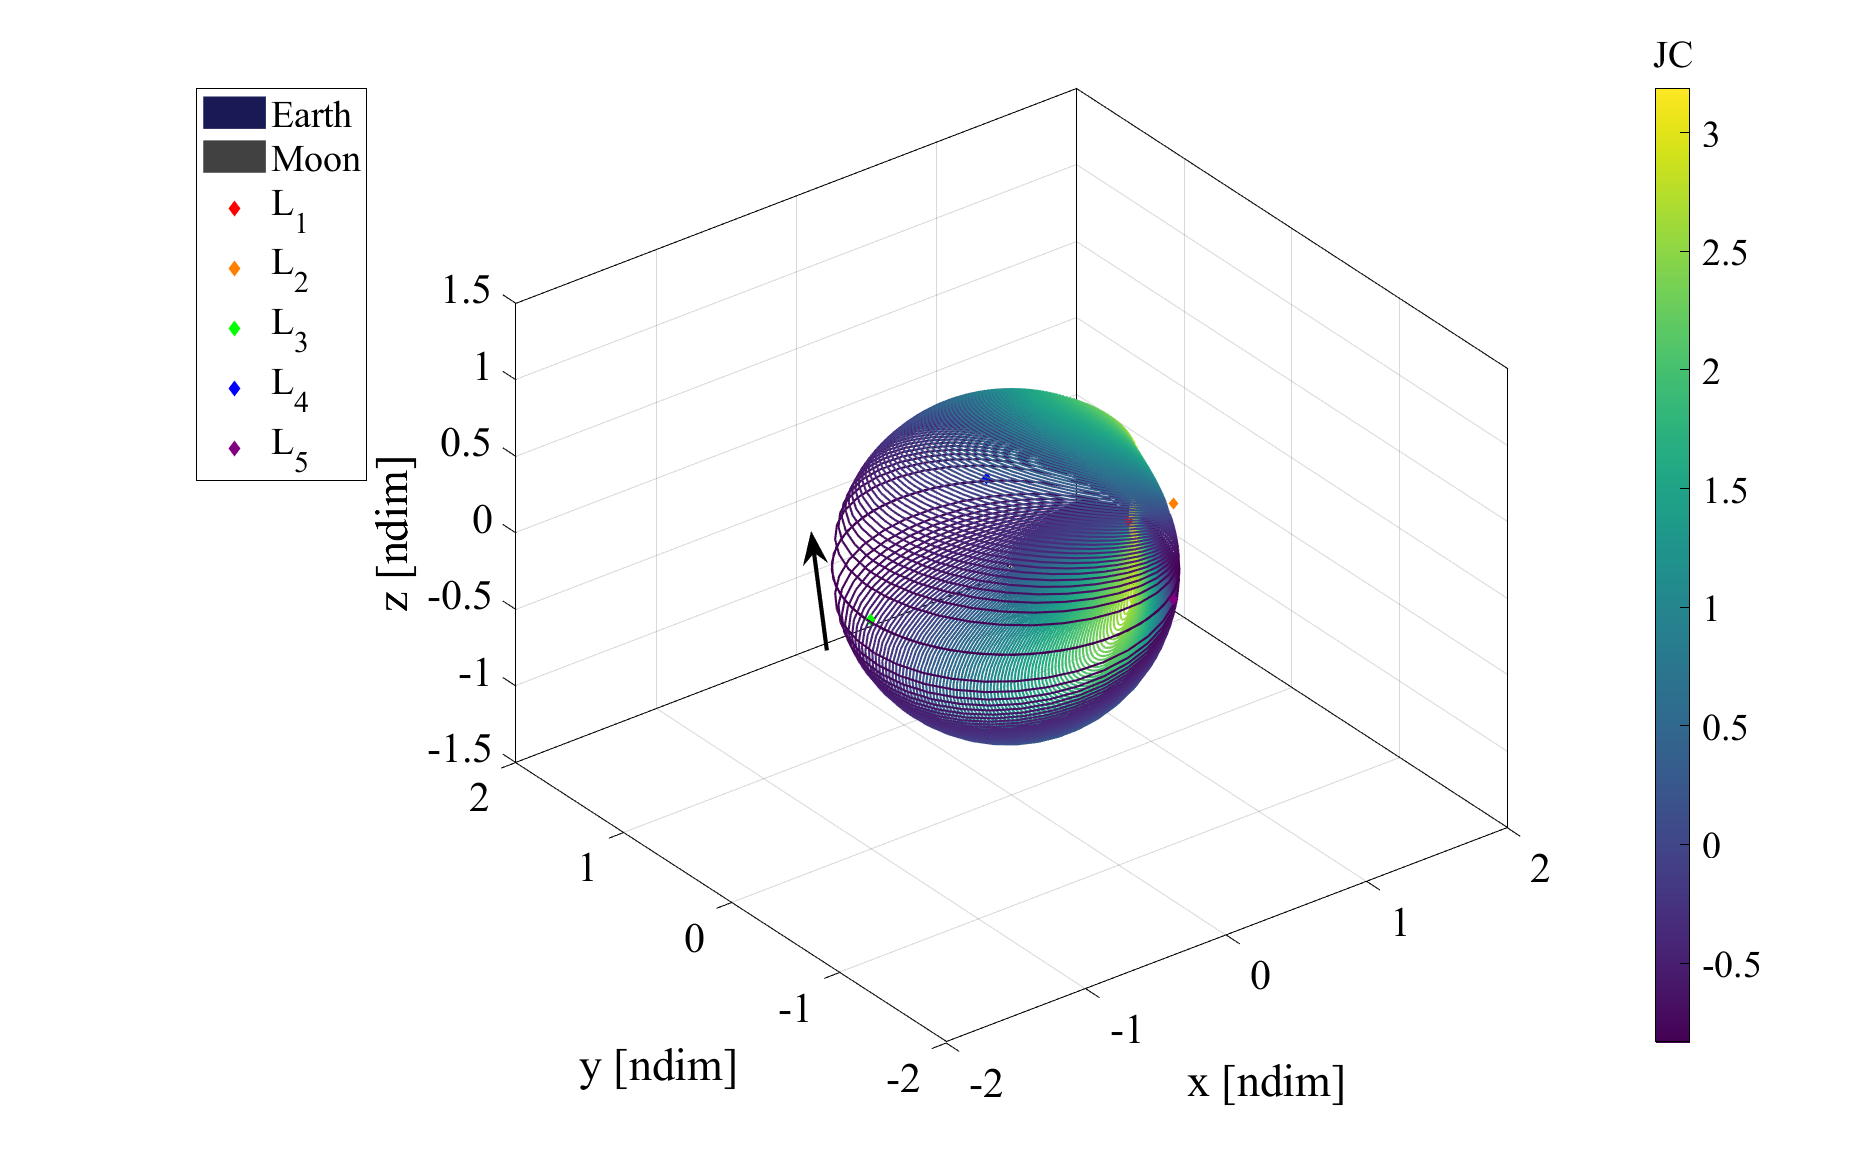
\includegraphics[width=0.9\textwidth]{figures/L1VerticalFamily.pdf}
    \caption{Earth-Moon $L_{1}$ vertical orbit family.}
    \label{fig:L1Vertical}
\end{figure}

\begin{figure}[ht]
    \centering
    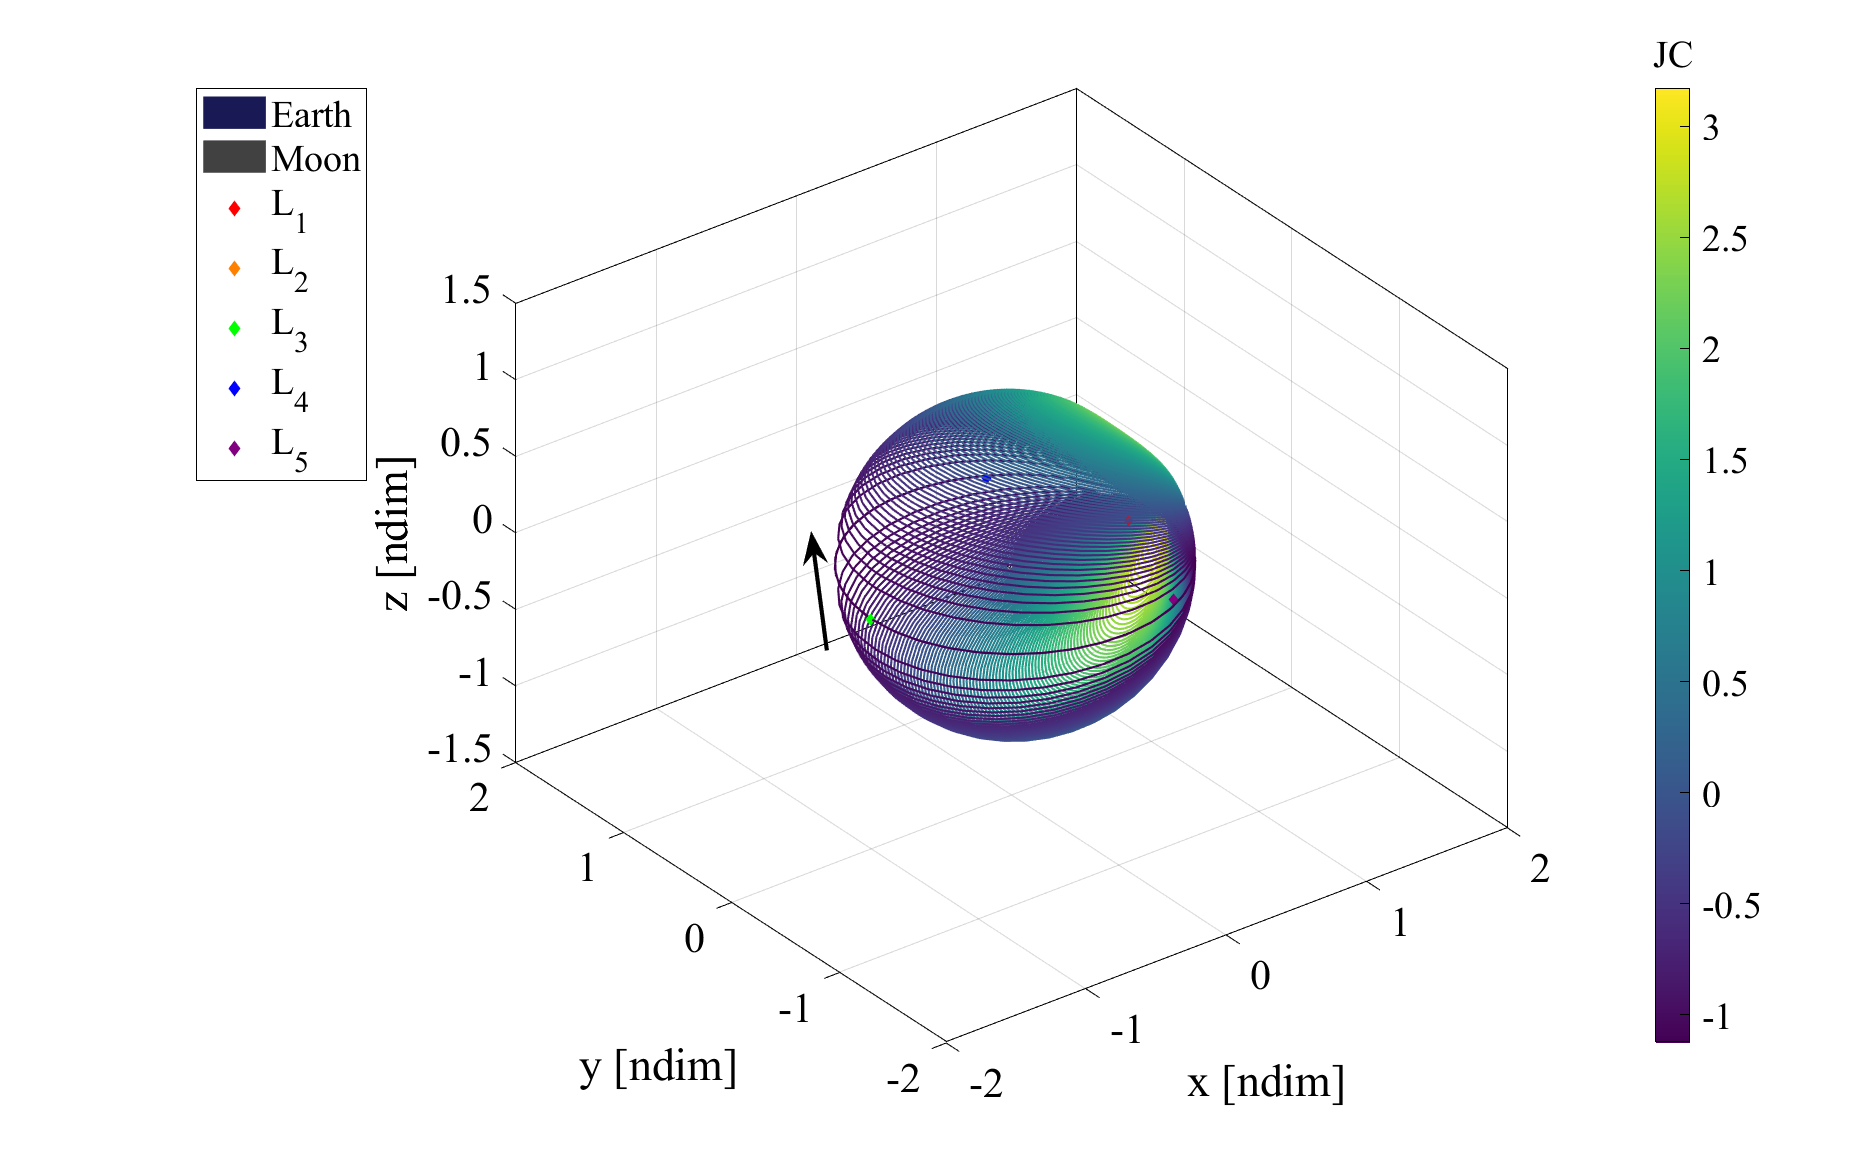
\includegraphics[width=0.9\textwidth]{figures/L2VerticalFamily.pdf}
    \caption{Earth-Moon $L_{2}$ vertical orbit family.}
    \label{fig:L2Vertical}
\end{figure}

\begin{figure}[ht]
    \begin{subfigure}[h]{0.4\linewidth}
        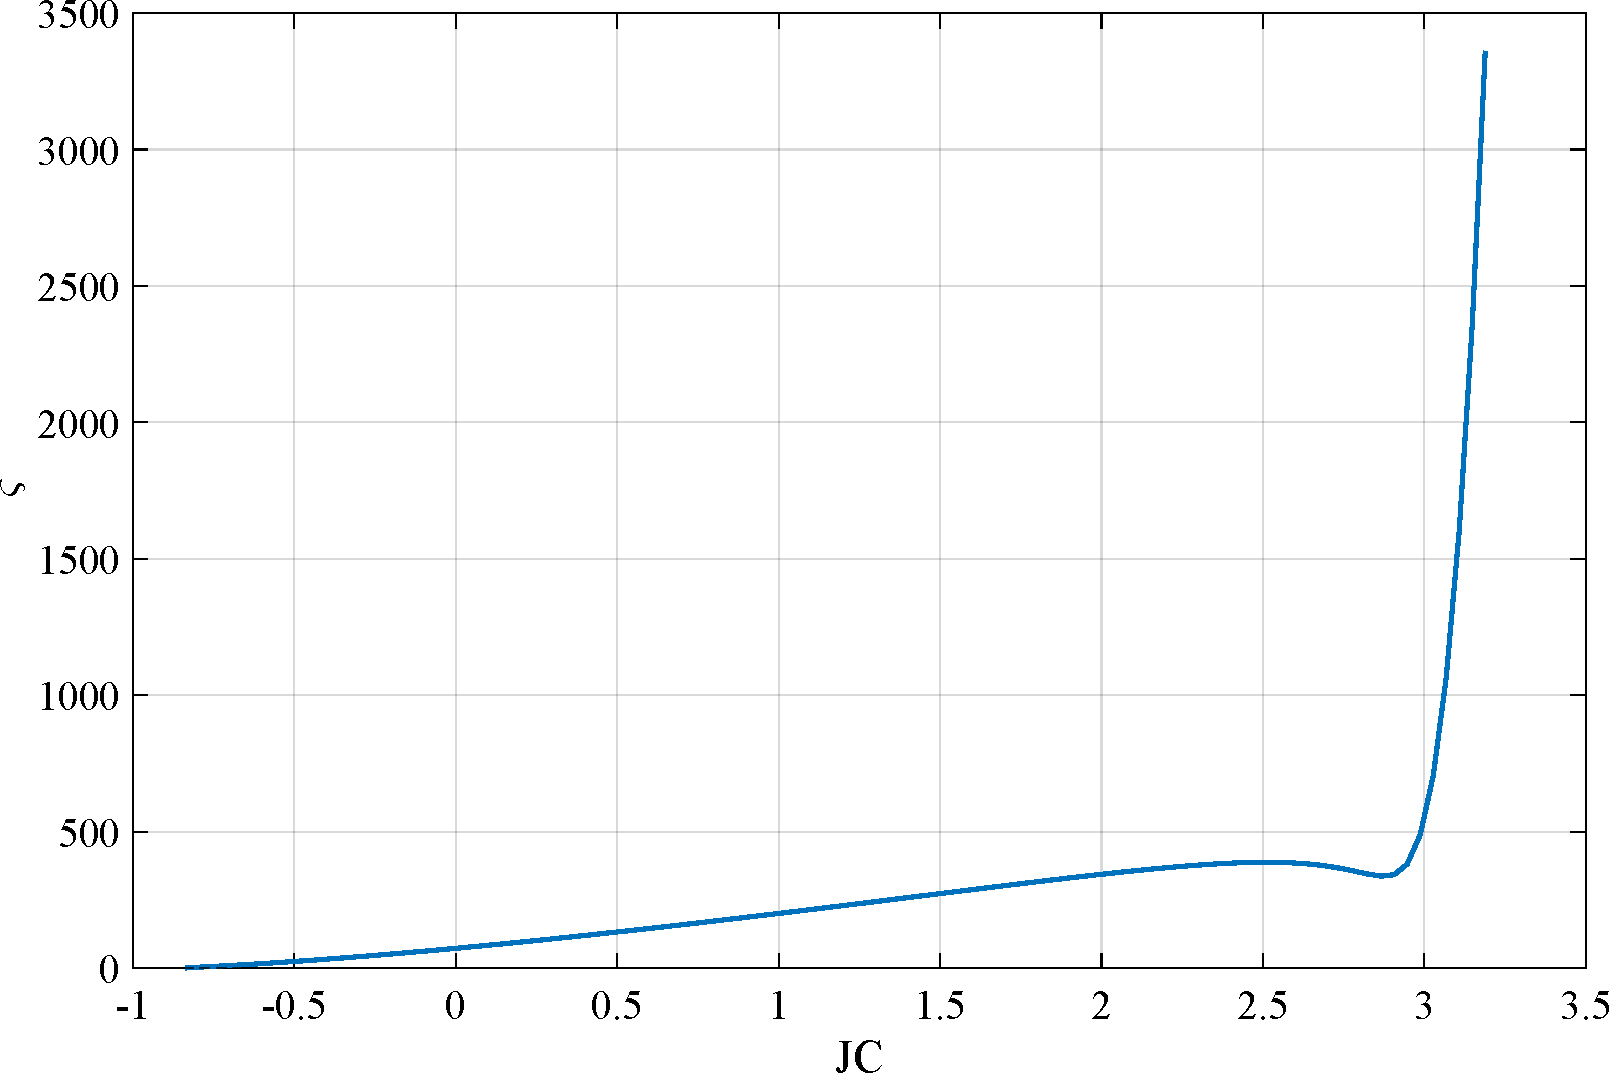
\includegraphics[width=\textwidth]{figures/L1VerticalStability.pdf}
        \caption{$L_{1}$}
    \end{subfigure}
    \hfill
    \begin{subfigure}[h]{0.4\linewidth}
        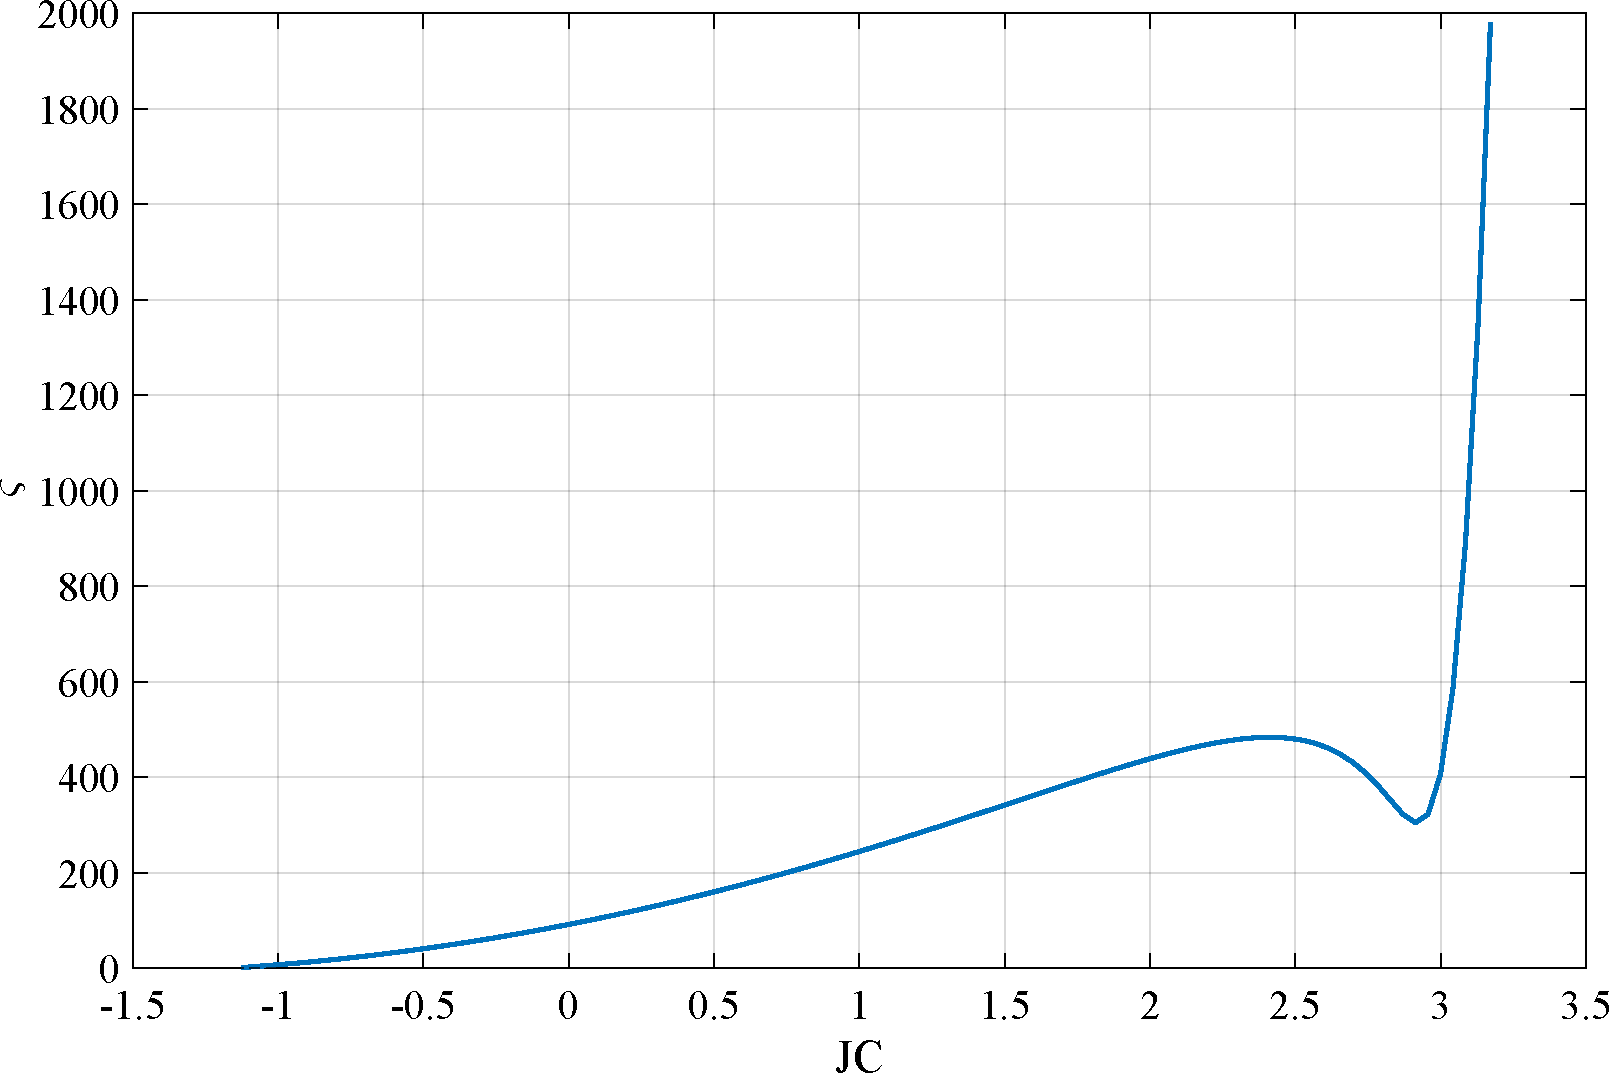
\includegraphics[width=\textwidth]{figures/L2VerticalStability.pdf}
        \caption{$L_{2}$}
    \end{subfigure}
    \caption{Earth-Moon vertical family stability index evolution.}
    \label{fig:verticalStability}
\end{figure}

\subsection{Equilateral Long Period Orbits}
\phantomsection
\subsubsection{A Planar Equilateral Orbit Targeter}
Similar to the Lyapunov orbits around the colinear equilibrium points, there are planar orbits
around the equilateral equilibrium points $L_{4}$ and $L_{5}$; however, they do not have symmetry
that can be exploited. Therefore, the full period of the orbit needs to be targeted, constraining
periodicity between the propagation start and end points. Note that since the Jacobi constant of a
propagated trajectory is naturally constrained, constraining periodicity only requires constraining
five out of the six states (three out of the four for a planar problem):
\begin{equation}
    \Xbar=\begin{bmatrix}   x_{0}   &   \xdot_{0}   &   \ydot_{0}   &   \tau    \end{bmatrix}^{T},
    \label{eq:longfreevar}
\end{equation}
\begin{equation}
    \Fbar(\Xbar)=\begin{bmatrix}    x_{f}-x_{0} &   y_{f}-y_{0} &   \xdot_{f}-\xdot_{0} &   C-C_{d} \end{bmatrix}^{T}=\zerobar,
    \label{eq:longconst}
\end{equation}
\begin{equation}
    DF(\Xbar)=\begin{bmatrix}   \phi_{11}-1                                                                 &   \phi_{14}   &   \phi_{15}   &   \xdot_{f}   \\
                                \phi_{21}                                                                   &   \phi_{24}   &   \phi_{25}   &   \ydot_{f}   \\
                                \phi_{41}                                                                   &   \phi_{44}-1 &   \phi_{45}   &   \xddot_{f}  \\
                                2x_{0}-\frac{2(x_{0}+\mu)(1-\mu)}{d^{3}}-\frac{2\mu(x_{0}-1+\mu)}{r^{3}}    &   -2\xdot_{0} &   -2\ydot_{0} &   0           \end{bmatrix}.
    \label{eq:longjacobian}
\end{equation}
Since $z=\zdot=0$, this targeter provides five of the six initial state variables and the full
period for the planar equilateral orbit.

\subsubsection{Long Period Equilateral Orbit Initial Guess}
Initial guesses for the planar equilateral orbits close to the Lagrange point can come from linear
variational equations of motion about the equilibrium point:
\begin{equation}
    x_{0}=x_{L}+\xi,
    \label{eq:xvareq}
\end{equation}
\begin{equation}
    y_{0}=y_{L}+\eta,
    \label{eq:yvareq}
\end{equation}
\begin{equation}
    \xdot_{0}=\alpha s,
    \label{eq:xdotvareq}
\end{equation}
\begin{equation}
    \ydot_{0}=\beta s,
    \label{eq:ydotvareq}
\end{equation}
where $\xi$ and $\eta$ are chosen variations from the Lagrange point,
\begin{equation}
    s=\Im(\lambda),
    \label{eq:seq}
\end{equation}
\begin{equation}
    \alpha=\frac{\xi\frac{\partial U}{\partial x\partial y}+\eta(\frac{\partial u}{\partial y\partial y}+s^{2})}{2s},
    \label{eq:alphaeq}
\end{equation}
\begin{equation}
    \beta=-\frac{\xi(\frac{\partial U}{\partial x\partial x}+s^{2})+\eta\frac{\partial U}{\partial x\partial y}}{2s}.
    \label{eq:betaeq}
\end{equation}
The linearization has two frequencies, short and long, and the choice of frequency determines
$\lambda$. The short period orbits are not used in this investigation, so for long period orbits:
\begin{equation}
    \lambda=\sqrt{\frac{\sqrt{1-27\mu(1-\mu)}-1}{2}}.
    \label{eq:lambdaeq}
\end{equation}

For consistency, $y_{0}$ is chosen to be the $y$-value of the Lagrange point $y_{L}$ with $\eta=0$.
The initial guess for the period is also determined by the choice of frequency:
\begin{equation}
    \tau=2\pi s.
    \label{eq:taueq}
\end{equation}

\subsubsection{Converged Equilateral Long Period Orbit Families}
Since the CR3BP is symmetric about the $xz$-plane, all $L_{4}$ orbit families can be mirrored
across that plane to find the $L_{5}$ families and vice versa. This is done by flipping the signs
of $y$, $\xdot$, and $\zdot$. Therefore, \cref{fig:longPeriod} shows portions of both equilateral
long period orbit families in the Earth-Moon system and \cref{fig:longPeriodStability} shows their
stability indices. 

\begin{figure}[ht]
    \centering
    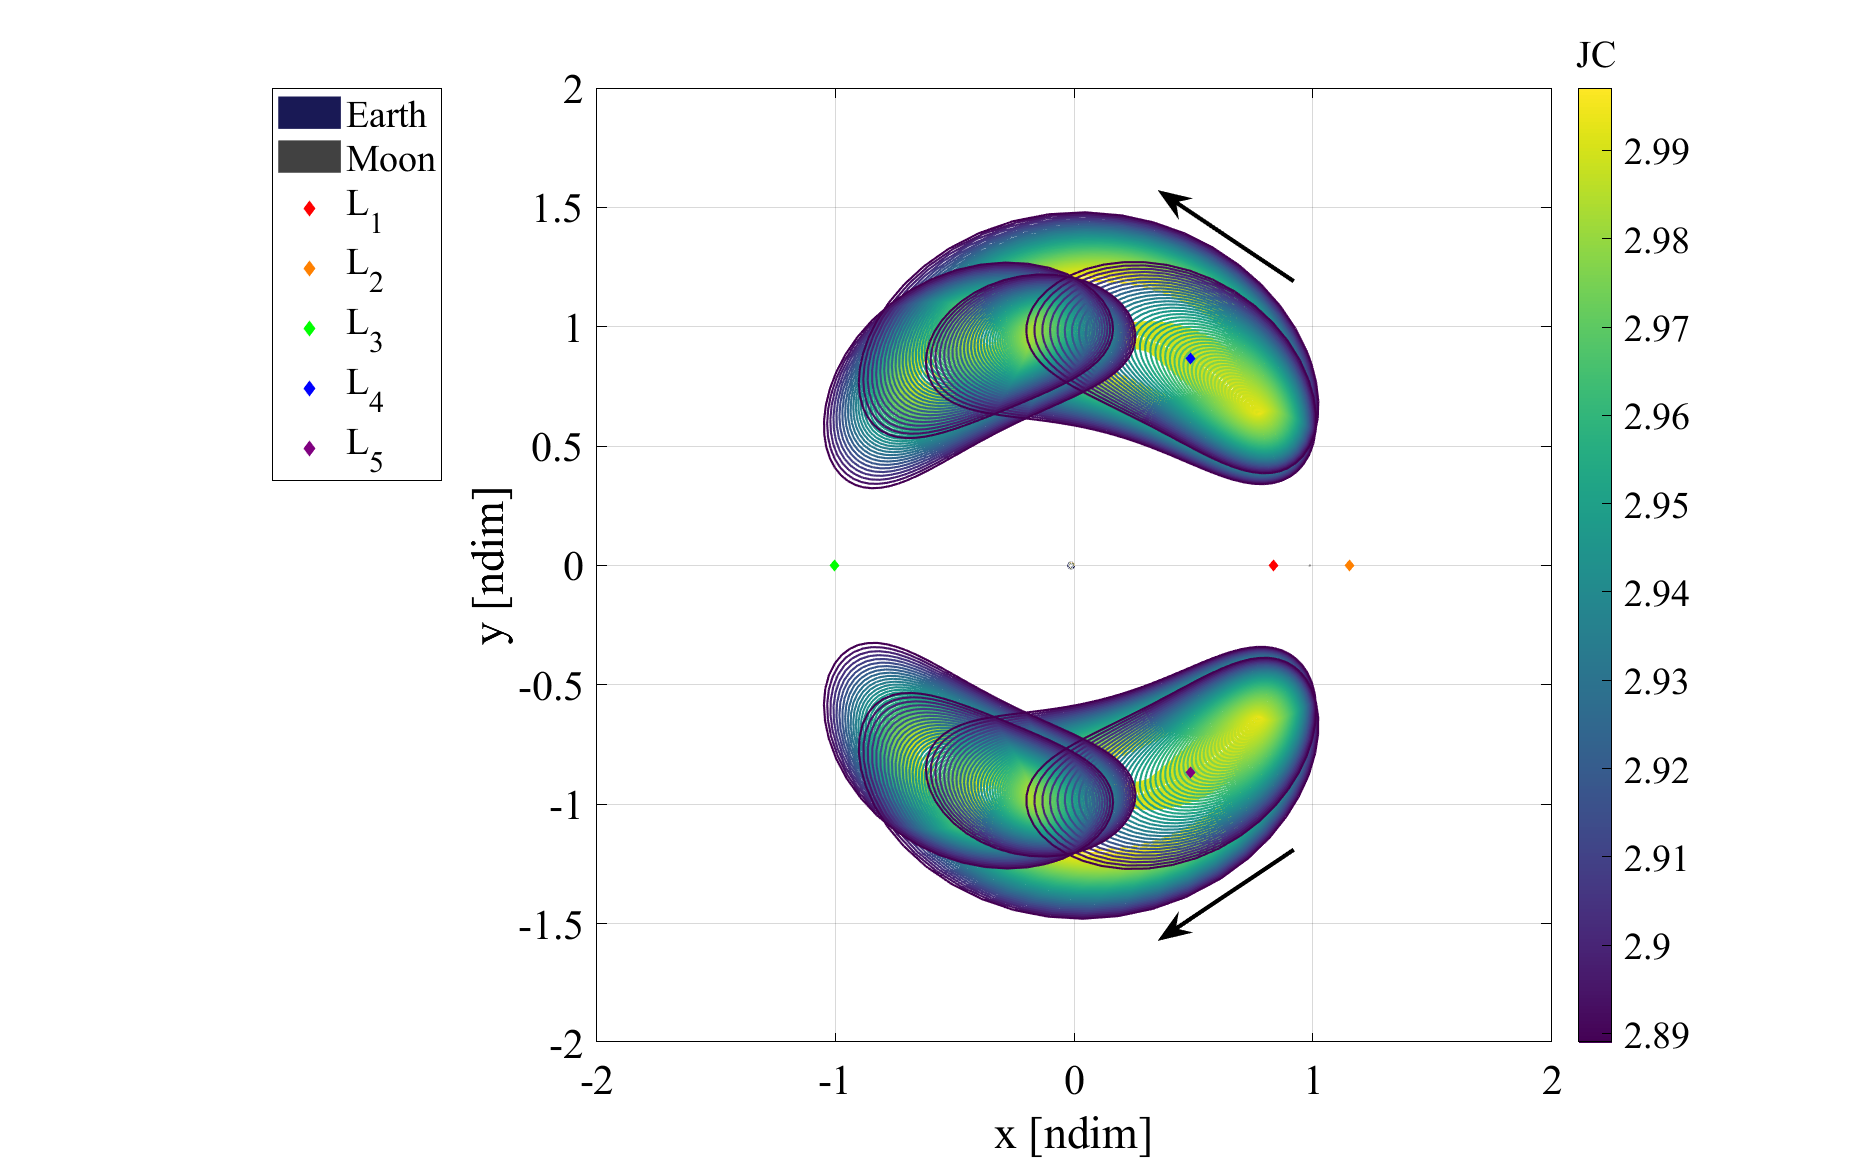
\includegraphics[width=0.9\textwidth]{figures/LongPeriodFamily.pdf}
    \caption{Earth-Moon $L_{4}$ and $L_{5}$ equilateral long period orbit families.}
    \label{fig:longPeriod}
\end{figure}

\begin{figure}[ht]
    \centering
    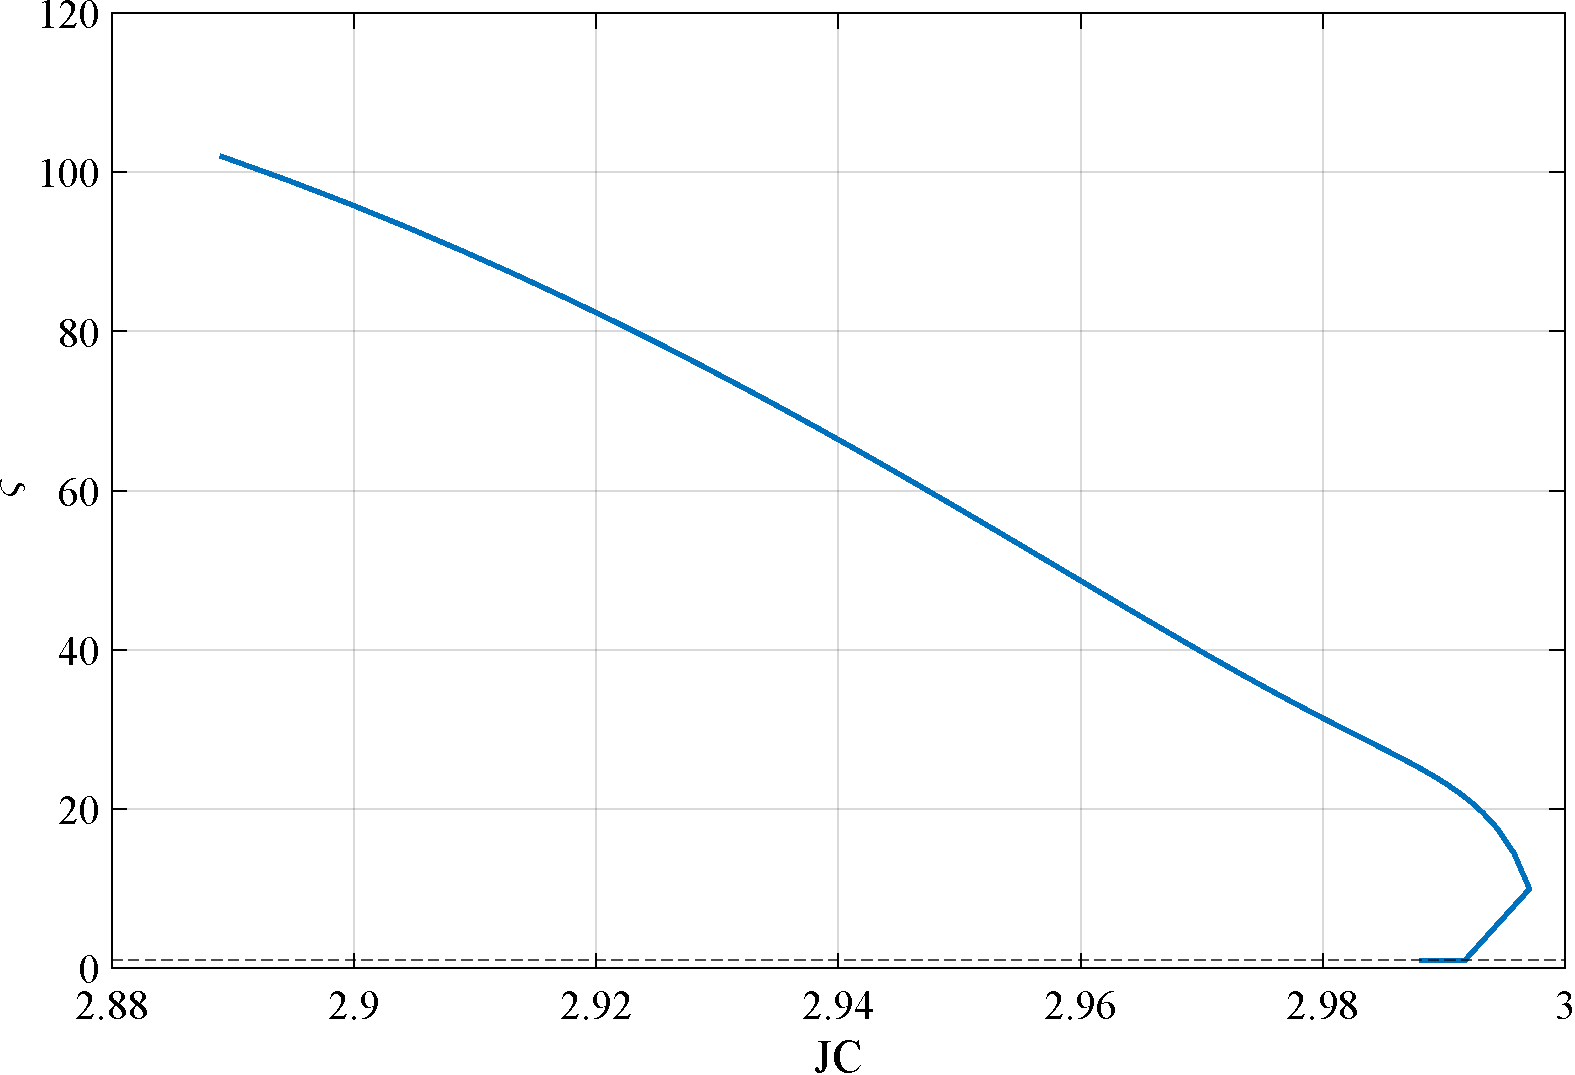
\includegraphics[width=0.5\textwidth]{figures/LongPeriodStability.pdf}
    \caption{Earth-Moon equilateral long period orbit family stability index evolution.}
    \label{fig:longPeriodStability}
\end{figure}

\subsection{Equilateral Axial Orbits}
\phantomsection
\subsubsection{A Spatial Equilateral Orbit Targeter}
While axial orbits exist around $L_{4}$ and $L_{5}$, unlike their colinear counterparts, these
axial families bifurcate from the $L_{1}$ halo family. Like the planar equilateral orbits, symmetry
cannot be exploited to aid the targeting process, so periodicity must be targeted instead:
\begin{equation}
    \Xbar=\begin{bmatrix}   x_{0}   &   y_{0}   &   \xdot_{0}   &   \ydot_{0}   &   \zdot_{0}   \tau    \end{bmatrix}^{T},
    \label{eq:eqaxialfreevar}
\end{equation}
\begin{equation}
    \Fbar(\Xbar)=\begin{bmatrix}    x_{f}-x_{0} &   y_{f}-y_{0} &   \xdot_{f}-\xdot_{0} &   \ydot_{f}-\ydot_{0} &   \zdot_{f}-\zdot_{0} &   C-C_{d} \end{bmatrix}^{T}=\zerobar,
    \label{eq:eqaxialconst}
\end{equation}
\begin{multline}
    DF(\Xbar)=\\
    \begin{bmatrix} \phi_{11}-1                                                                 &   \phi_{12}                                                   &   \phi_{14}   &   \phi_{15}   &   \phi_{16}   &   \xdot_{f}   \\
                    \phi_{21}                                                                   &   \phi_{22}-1                                                 &   \phi_{24}   &   \phi_{25}   &   \phi_{26}   &   \ydot_{f}   \\
                    \phi_{41}                                                                   &   \phi_{42}                                                   &   \phi_{44}-1 &   \phi_{45}   &   \phi_{46}   &   \xddot_{f}  \\
                    \phi_{51}                                                                   &   \phi_{52}                                                   &   \phi_{54}   &   \phi_{55}-1 &   \phi_{56}   &   \yddot_{f}  \\
                    \phi_{61}                                                                   &   \phi_{62}                                                   &   \phi_{64}   &   \phi_{65}   &   \phi_{66}-1 &   \zddot_{f}  \\
                    2x_{0}-\frac{2(x_{0}+\mu)(1-\mu)}{d^{3}}-\frac{2\mu(x_{0}-1+\mu)}{r^{3}}    &   2y_{0}-\frac{2y_{0}(1-\mu)}{d^{3}}-\frac{2y_{0}\mu}{r^{3}}  &   -2\xdot_{0} &   -2\ydot_{0} &   -2\zdot_{0} &   0           \end{bmatrix}.
    \label{eq:eqaxialjacobian}
\end{multline}

\subsubsection{Converged Equilateral Axial Families}
The pseudo-arclength method can be used to obtain the initial guess for the equilateral axial
family. Stepping in one direction will produce the $L_{4}$ family, while stepping in the other
produces the $L_{5}$ family. These are both shown in \cref{fig:eqAxial}.
\cref{fig:eqAxialStability} shows the stability indices for these family. As hinted at by the end
of these axial families, $L_{4}$ and $L_{5}$ vertical families also exist in the Earth-Moon system,
but are not used in this investigation.

\begin{figure}[ht]
    \centering
    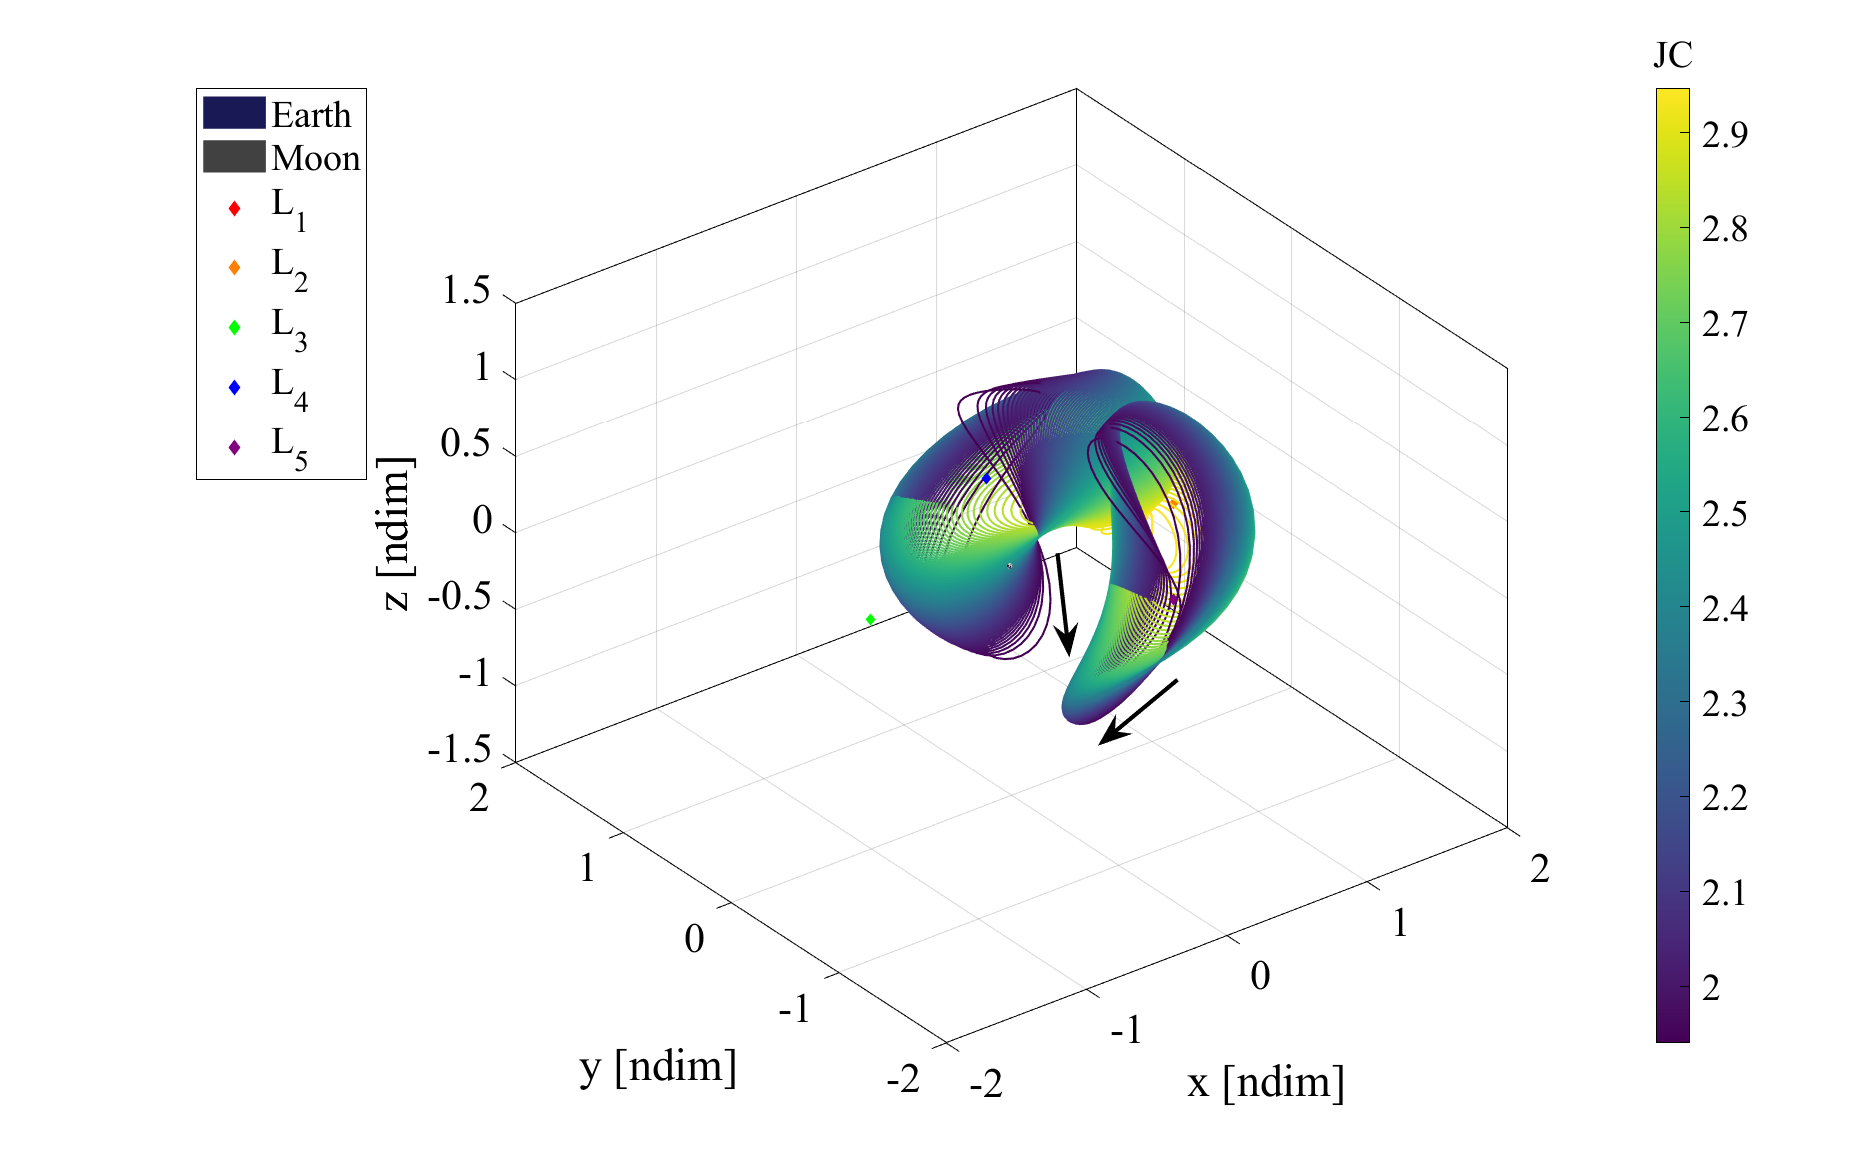
\includegraphics[width=0.9\textwidth]{figures/EquilateralAxialFamily.pdf}
    \caption{Earth-Moon $L_{4}$ and $L_{5}$ equilateral axial families.}
    \label{fig:eqAxial}
\end{figure}

\begin{figure}[ht]
    \centering
    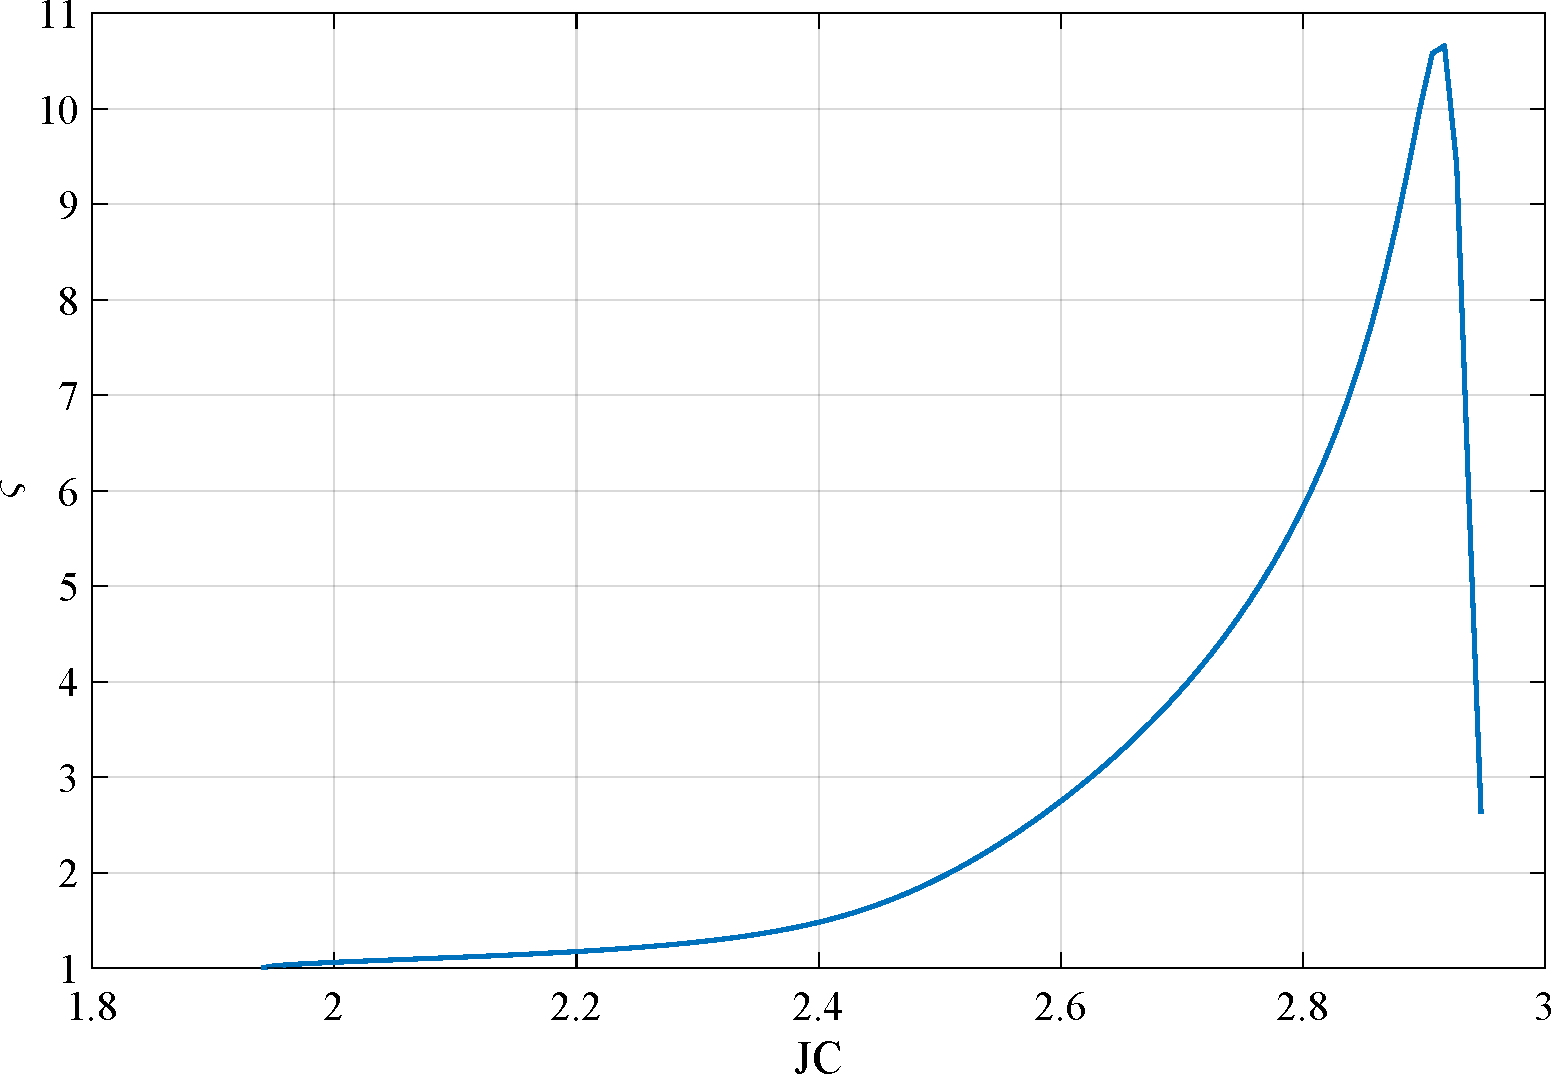
\includegraphics[width=0.5\textwidth]{figures/EquilateralAxialStability.pdf}
    \caption{Earth-Moon equilateral axial family stability index evolution.}
    \label{fig:eqAxialStability}
\end{figure}

\subsection{Resonant Orbits}
There are many other types of CR3BP orbits that are not associated with a Lagrange point. Some of
these orbit families are known as resonant orbits because their periods are resonant or close to
resonant with the Moon's' period. These orbits are still periodic in the rotating frame but are
also periodic or close to periodic in an inertial frame. Individual orbits also tend to span more
of the Earth-Moon system than the Lagrange point orbits. For more details on how to determine
initial guesses and correct these orbits, Gupta\cite{Gupta:2020} and Sadaka\cite{Sadaka:2023}
provide extensive overviews and initial conditions. A couple of unstable resonant orbit families
are used in this investigation and so they are shown here.

\phantomsection
\subsubsection{Converged 2:1a Resonant Orbit Family}
The unstable section of the 2:1 resonant orbit family (denoted the 2:1a resonant orbit family by
Sadaka) is shown in \cref{fig:2_1aResonant}\cite{Sadaka:2023}. These orbits travel around the
Earth roughly twice for every time the Moon revolves around it, which becomes more evident when
the trajectories are viewed in an inertial frame. \cref{fig:2_1aResonantStability} shows the
stability index evolution for this family.

\begin{figure}[ht]
    \centering
    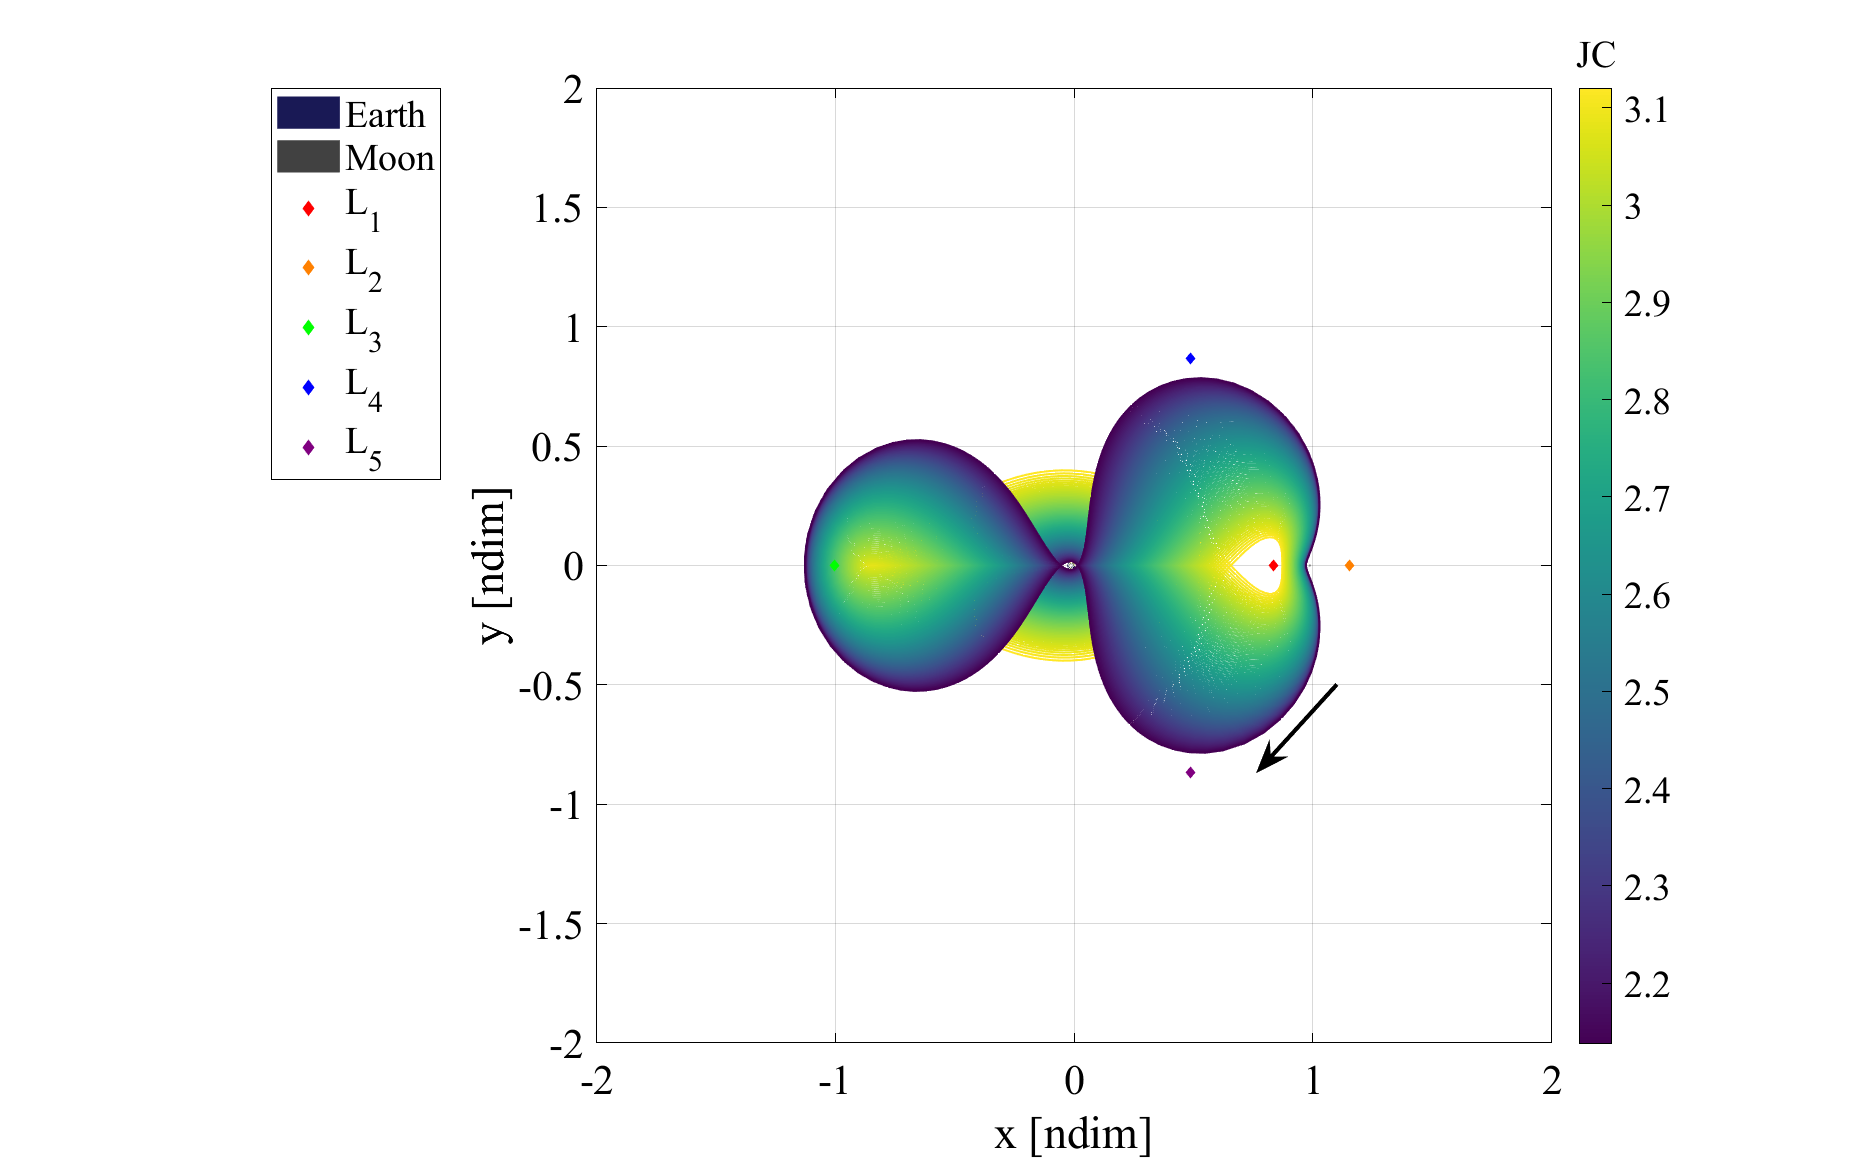
\includegraphics[width=0.9\textwidth]{figures/Resonant2_1aFamily.pdf}
    \caption{Earth-Moon 2:1a resonant orbit family.}
    \label{fig:2_1aResonant}
\end{figure}

\begin{figure}[ht]
    \centering
    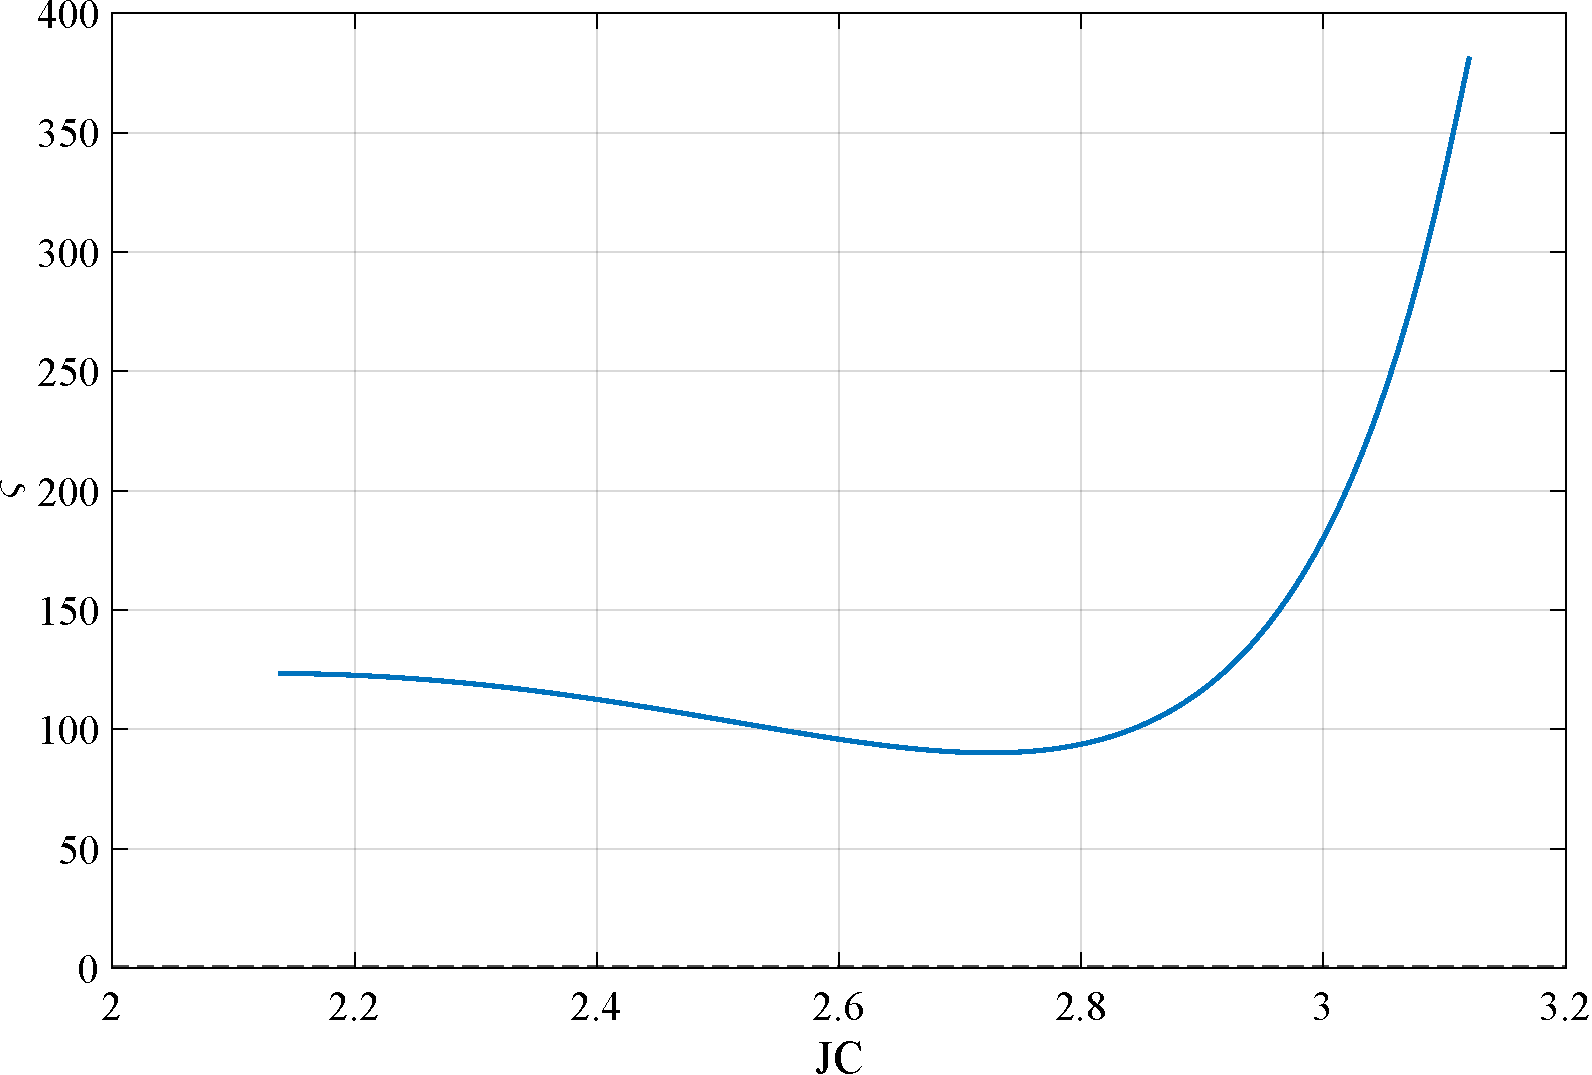
\includegraphics[width=0.5\textwidth]{figures/Resonant2_1aStability.pdf}
    \caption{Earth-Moon 2:1a resonant orbit family stability index evolution.}
    \label{fig:2_1aResonantStability}
\end{figure}

\subsubsection{Converged 3:4 Resonant Orbit Family}
Another unstable family is the 3:4 resonant orbits, shown in \cref{fig:3_4Resonant}. These orbits
go around the Earth three times for every times the Moon goes around. Their stability indices are
given in \cref{fig:3_4ResonantStability}.

\begin{figure}[ht]
    \centering
    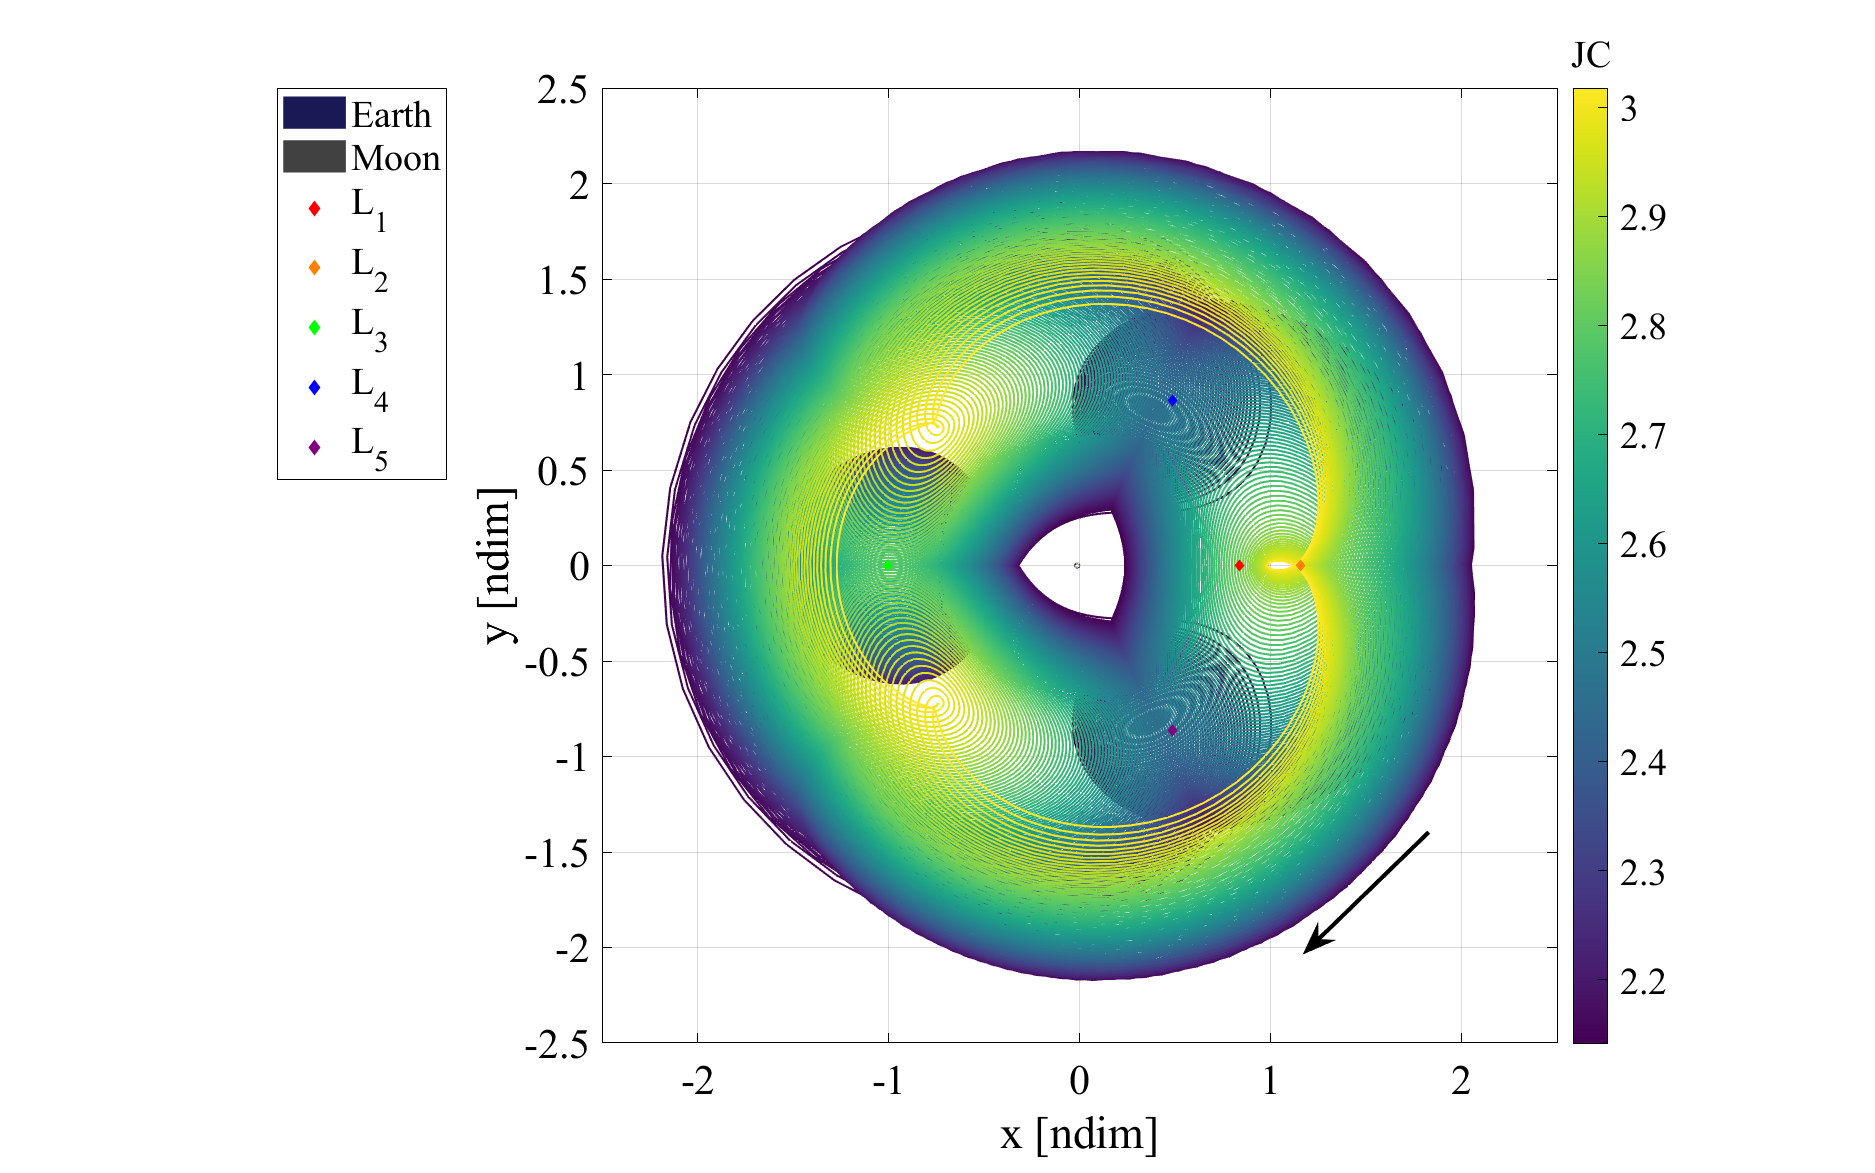
\includegraphics[width=0.9\textwidth]{figures/Resonant3_4Family.pdf}
    \caption{Earth-Moon 3:4 resonant orbit family.}
    \label{fig:3_4Resonant}
\end{figure}

\begin{figure}[ht]
    \centering
    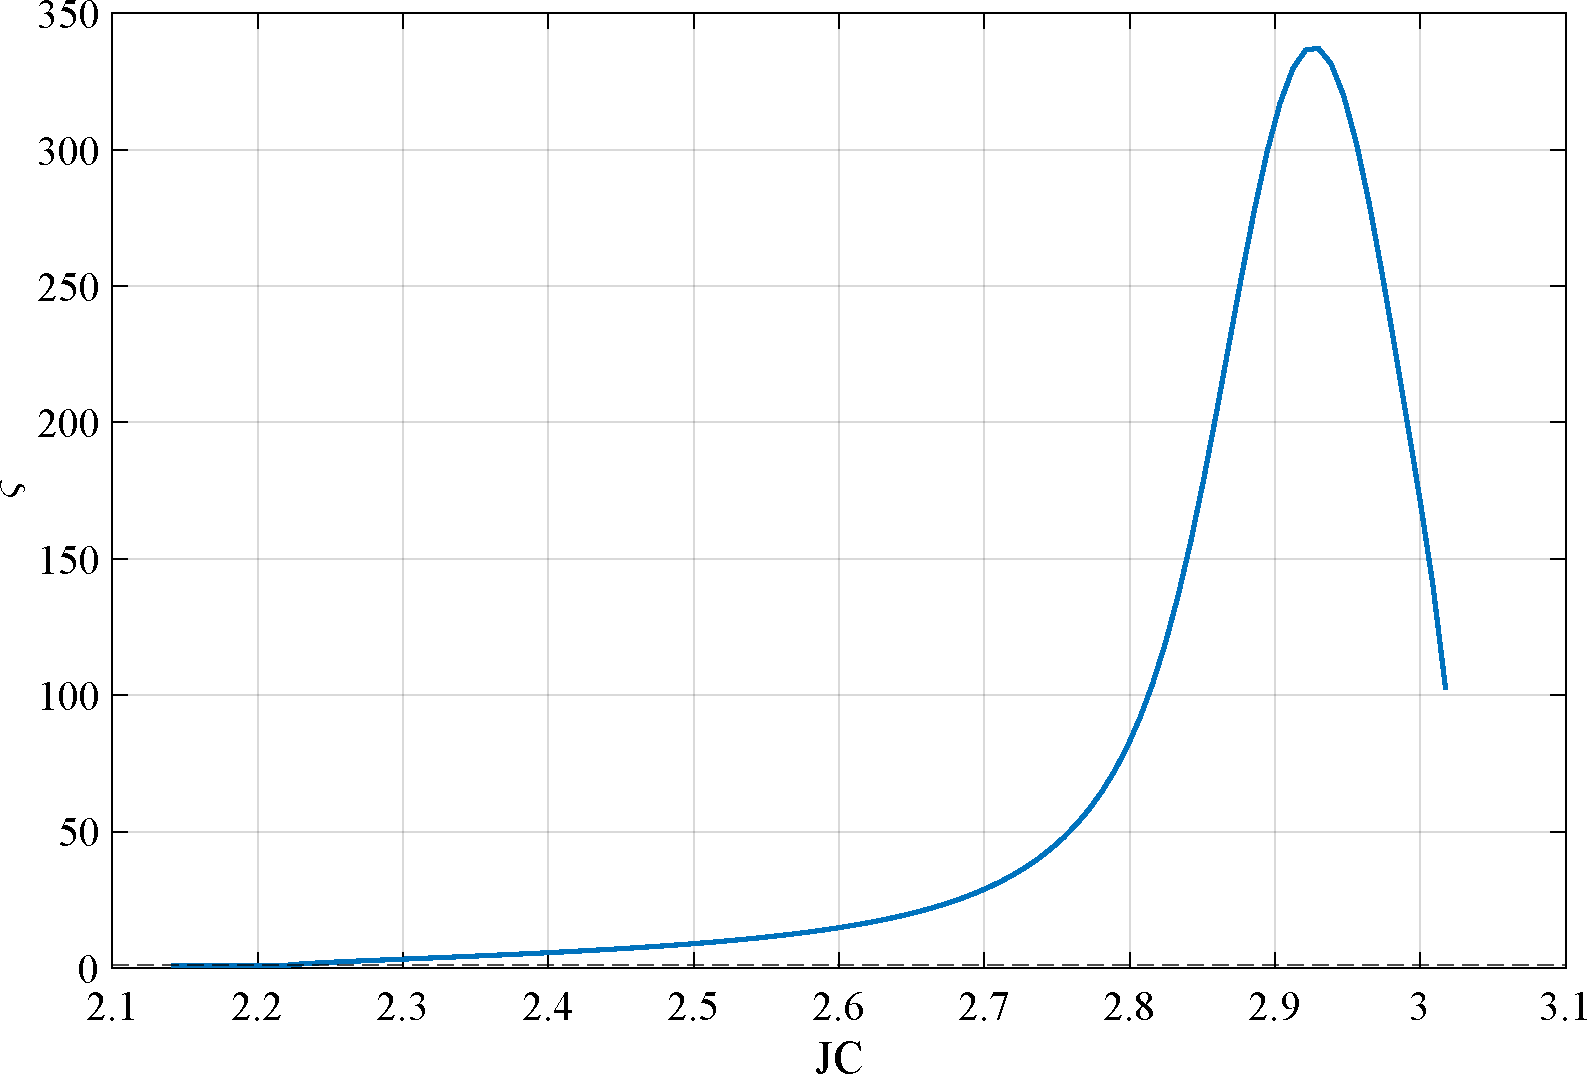
\includegraphics[width=0.5\textwidth]{figures/Resonant3_4Stability.pdf}
    \caption{Earth-Moon 3:4 resonant orbit family stability index evolution.}
    \label{fig:3_4ResonantStability}
\end{figure}
